\section{CPU Testing}
\textbf{Выданные параметры:} [fft,cdouble]\\
\textbf{Параметры процессора используемого в тесте:}\\
{\large Intel Core i5-8259U}\\
Ядер: 4\\
Потоков: 8\\
Базовая частота: 	2.30 ГГц\\
Кэш 1-го уровня: 	64K (на ядро)\\
Кэш 2-го уровня: 	256K (на ядро)\\
Кэш 3-го уровня: 	6 Мб (всего)\\
Входе теста используется ОС Linux установленная на виртуальную машину через Parallels.\\
Ограничение по процессорам: 8\\
Ограничение по памяти: 2048 MB\\
\subsection{fft}
\subsubsection{Команда lscpu}
\begin{verbatim}
  Architecture:            x86_64
  CPU op-mode(s):        32-bit, 64-bit
  Address sizes:         36 bits physical, 48 bits virtual
  Byte Order:            Little Endian
CPU(s):                  8
  On-line CPU(s) list:   0-7
Vendor ID:               GenuineIntel
  Model name:            Intel(R) Core(TM) i5-8259U CPU @ 2.30GHz
    CPU family:          6
    Model:               142
    Thread(s) per core:  1
    Core(s) per socket:  8
    Socket(s):           1
    Stepping:            10
    BogoMIPS:            4608.00
    Flags:               fpu vme de pse tsc msr pae mce cx8 apic sep mtrr pge mc
                         a cmov pat pse36 clflush mmx fxsr sse sse2 ss ht syscal
                         l nx rdtscp lm constant_tsc nopl xtopology nonstop_tsc 
                         cpuid tsc_known_freq pni pclmulqdq ssse3 fma cx16 pcid 
                         sse4_1 sse4_2 x2apic movbe popcnt tsc_deadline_timer ae
                         s xsave avx f16c rdrand hypervisor lahf_lm abm 3dnowpre
                         fetch invpcid_single pti fsgsbase tsc_adjust bmi1 avx2 
                         smep bmi2 invpcid rdseed adx smap clflushopt xsaveopt x
                         savec dtherm arat pln pts
Virtualization features: 
  Hypervisor vendor:     KVM
  Virtualization type:   full
Caches (sum of all):     
  L1d:                   256 KiB (8 instances)
  L1i:                   256 KiB (8 instances)
  L2:                    2 MiB (8 instances)
  L3:                    6 MiB (1 instance)
NUMA:                    
  NUMA node(s):          1
  NUMA node0 CPU(s):     0-7
Vulnerabilities:         
  Gather data sampling:  Unknown: Dependent on hypervisor status
  Itlb multihit:         KVM: Mitigation: VMX unsupported
  L1tf:                  Mitigation; PTE Inversion
  Mds:                   Vulnerable: Clear CPU buffers attempted, no microcode; 
                         SMT Host state unknown
  Meltdown:              Mitigation; PTI
  Mmio stale data:       Vulnerable: Clear CPU buffers attempted, no microcode; 
                         SMT Host state unknown
  Retbleed:              Vulnerable
  Spec rstack overflow:  Not affected
  Spec store bypass:     Vulnerable
  Spectre v1:            Mitigation; usercopy/swapgs barriers and __user pointer
                          sanitization
  Spectre v2:            Mitigation; Retpolines, STIBP disabled, RSB filling, PB
                         RSB-eIBRS Not affected
  Srbds:                 Unknown: Dependent on hypervisor status
  Tsx async abort:       Not affected

\end{verbatim}
Видим, что Linux распознает наши 4 ядра по 2 потока, как 8 ядер по 1 потоку.
\subsubsection{Команда lstopo}
С помощью команды lstopo мы можем посмотреть на топологию нашего процессора:\\
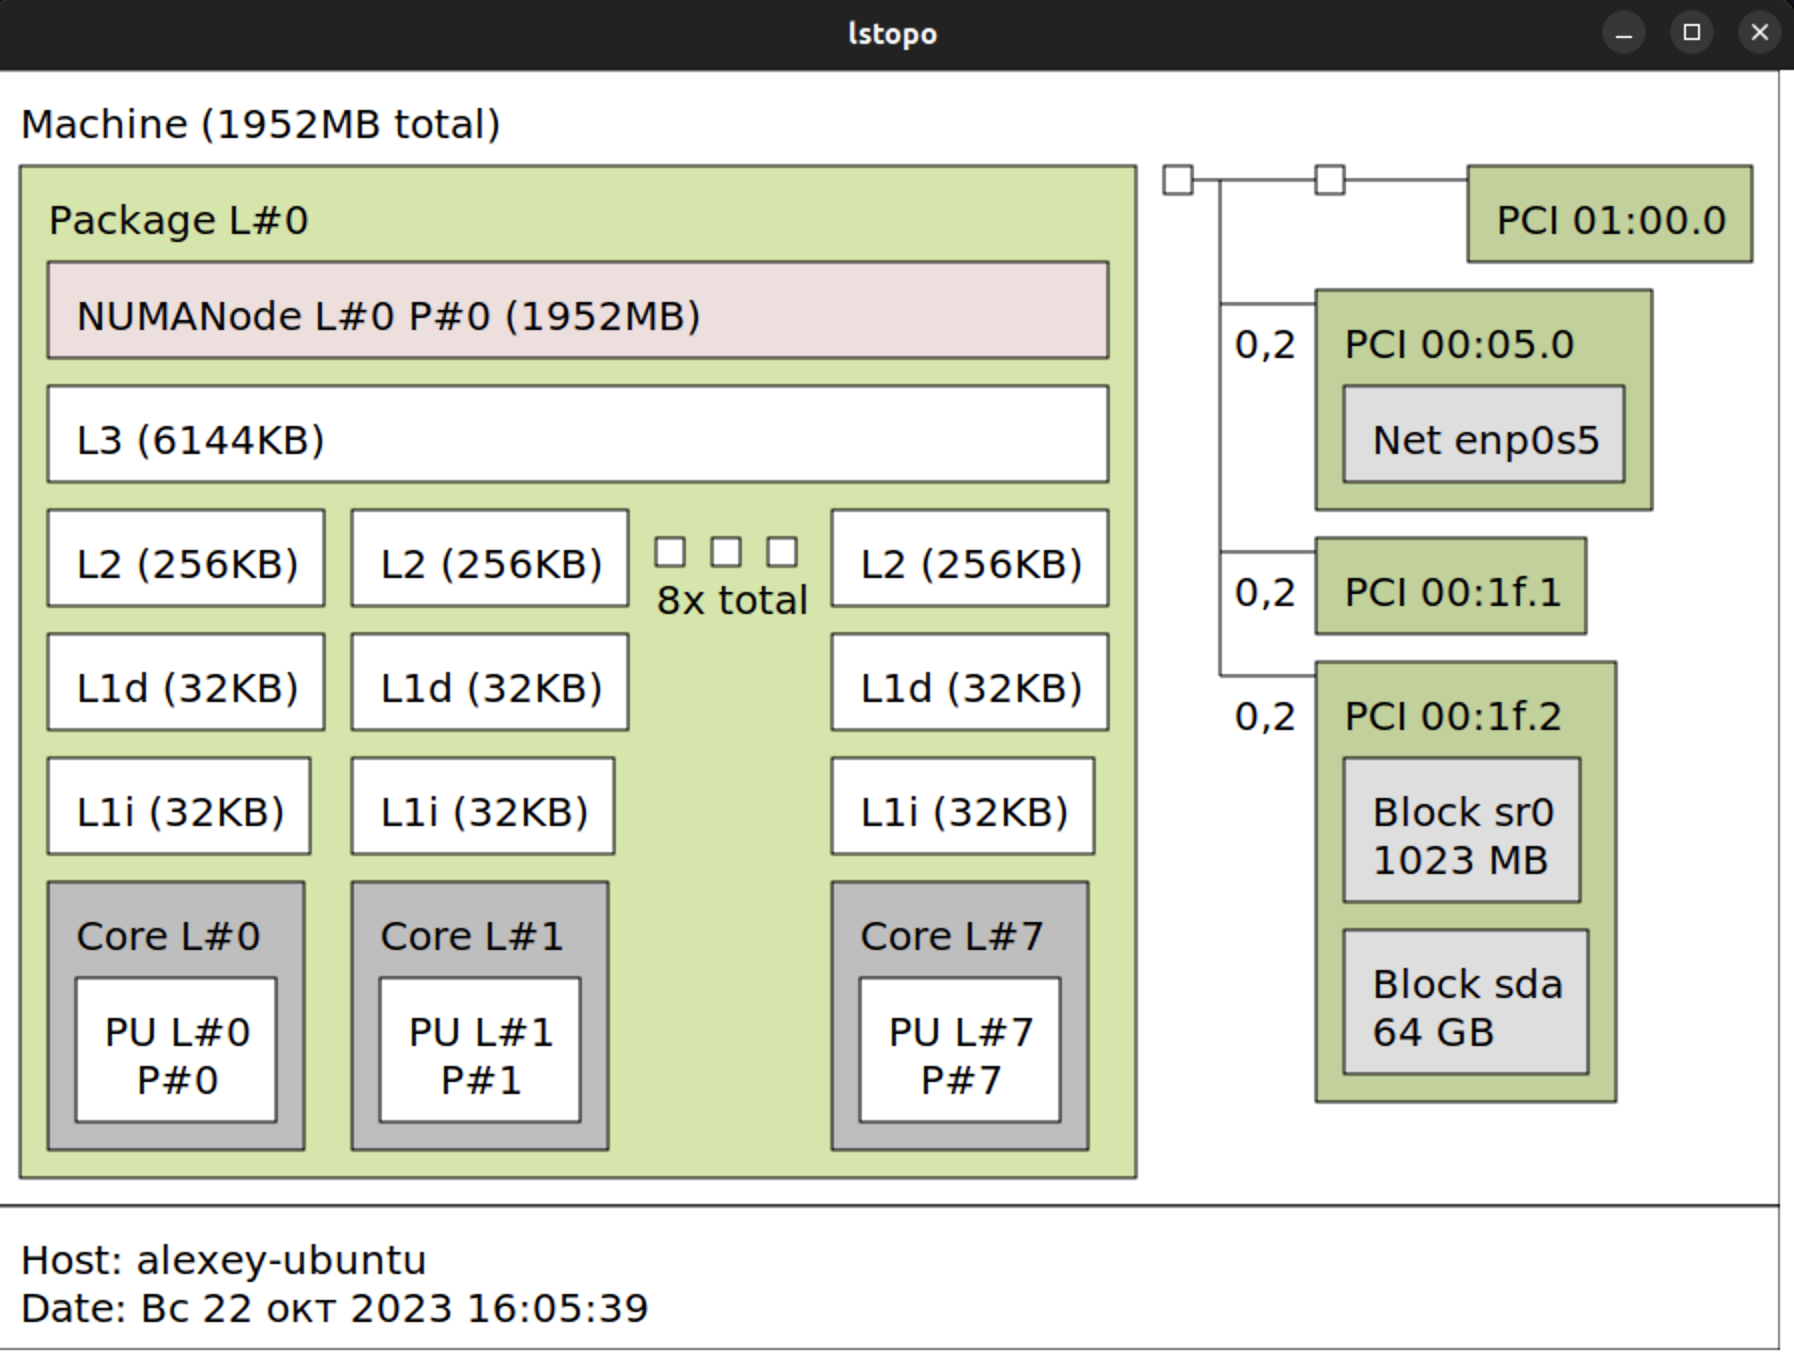
\includegraphics[width=\textwidth]{image/lstopo.png}
\subsubsection{Команда pidstat}
Посмосмотрим статистику по процессу\\
Для этого запустим команду: \textit{stress-ng --cpu 1 --cpu-method fft --metrics --timeout 120}\\
И посмотрим статистику запустив команду: \textit{pidstat -p 58452 1}, где pid мы узнали спомощью команды \textit{top}.
\begin{verbatim}
20:45:33      UID       PID    %usr %system  %guest   %wait    %CPU   CPU  Command
20:45:34     1000     58452  100,00    0,00    0,00    0,00  100,00     3  stress-ng
20:45:35     1000     58452  100,00    0,00    0,00    0,00  100,00     3  stress-ng
20:45:36     1000     58452  100,00    0,00    0,00    0,00  100,00     3  stress-ng
20:45:37     1000     58452  100,00    0,00    0,00    0,00  100,00     3  stress-ng
20:45:38     1000     58452  100,00    0,00    0,00    0,00  100,00     3  stress-ng
20:45:39     1000     58452   99,01    0,00    0,00    0,00   99,01     3  stress-ng
20:45:40     1000     58452  100,00    0,00    0,00    0,00  100,00     3  stress-ng
20:45:41     1000     58452  101,00    0,00    0,00    0,00  101,00     3  stress-ng
20:45:42     1000     58452  100,00    0,00    0,00    0,00  100,00     3  stress-ng
20:45:43     1000     58452  100,00    0,00    0,00    0,00  100,00     3  stress-ng
20:45:44     1000     58452   99,01    0,00    0,00    0,00   99,01     3  stress-ng
20:45:45     1000     58452  100,00    0,00    0,00    0,00  100,00     3  stress-ng
20:45:46     1000     58452  100,00    0,00    0,00    0,00  100,00     3  stress-ng
20:45:47     1000     58452  100,00    0,00    0,00    0,00  100,00     3  stress-ng
20:45:48     1000     58452  100,00    0,00    0,00    0,00  100,00     3  stress-ng
20:45:49     1000     58452  100,00    0,00    0,00    0,00  100,00     3  stress-ng
20:45:50     1000     58452  100,00    0,00    0,00    0,00  100,00     3  stress-ng
20:45:51     1000     58452  100,00    0,00    0,00    0,00  100,00     3  stress-ng
20:45:52     1000     58452  100,00    0,00    0,00    0,00  100,00     3  stress-ng
20:45:53     1000     58452  101,00    0,00    0,00    0,00  101,00     3  stress-ng
20:45:54     1000     58452  100,00    0,00    0,00    0,00  100,00     3  stress-ng
20:45:55     1000     58452  100,00    0,00    0,00    0,00  100,00     3  stress-ng
20:45:56     1000     58452   99,01    0,00    0,00    0,00   99,01     3  stress-ng
20:45:57     1000     58452  100,00    0,00    0,00    0,00  100,00     3  stress-ng
20:45:58     1000     58452  100,00    0,00    0,00    0,00  100,00     3  stress-ng
20:45:59     1000     58452  100,00    0,00    0,00    0,00  100,00     3  stress-ng
20:46:00     1000     58452  100,00    0,00    0,00    0,00  100,00     3  stress-ng
20:46:01     1000     58452  100,00    0,00    0,00    0,00  100,00     3  stress-ng
20:46:02     1000     58452  100,00    0,00    0,00    0,00  100,00     3  stress-ng
20:46:03     1000     58452  100,00    0,00    0,00    0,00  100,00     3  stress-ng
^C
Average:     1000     58452   99,97    0,00    0,00    0,00   99,97     -  stress-ng
\end{verbatim}
Мы видим, что процесс выполнялся на процессоре номер 3 и занимал почти все его время(100\%).
При этом процесс выполнялся практически все время в режиме \textit{пользователя}, что объяснимо так как fft - вычислительная задача.\\
Результат \textit{stress-ng}:
\lstconsolestyle
\definecolor{xxxhtmlcolorIMAIMP}{HTML}{26A269}
\definecolor{xxxhtmlcolorHIKOOB}{HTML}{12488B}
\begin{lstlisting}
%*{\color{xxxhtmlcolorIMAIMP}
  {\bfseries alexey@alexey{-}ubuntu}}*):%*{\color{xxxhtmlcolorHIKOOB}{\bfseries \textasciitilde{}}}*)$ stress-ng --cpu 1 --cpu-method fft --metrics --timeout 120

stress-ng: info:  [58451] setting to a 120 second (2 mins, 0.00 secs) run per stressor

stress-ng: info:  [58451] dispatching hogs: 1 cpu

stress-ng: info:  [58451] successful run completed in 120.00s (2 mins, 0.00 secs)

stress-ng: info:  [58451] stressor  bogo ops real time  usr time  sys time   bogo ops/s     bogo ops/s CPU used per

stress-ng: info:  [58451]                    (secs)    (secs)    (secs)   (real time) (usr+sys time) instance (%)

stress-ng: info:  [58451] cpu       102216    120.00    119.97      0.00       851.79         852.01        99.97
\end{lstlisting}

Также посмотрим на приоритет и политику планирования процесса: \\
{\lstconsolestyle
\definecolor{xxxhtmlcolorIMAIMP}{HTML}{26A269}
\definecolor{xxxhtmlcolorHIKOOB}{HTML}{12488B}\begin{lstlisting}
%*{\color{xxxhtmlcolorIMAIMP}{\bfseries alexey@alexey{-}ubuntu}}*):%*{\color{xxxhtmlcolorHIKOOB}{\bfseries \textasciitilde{}}}*)$ pidstat -R -p 76043 1

Linux 6.2.0-35-generic (alexey-ubuntu) 	22.10.2023 	_x86_64_	(8 CPU)



22:28:20      UID       PID     prio policy  Command

22:28:21   %*{\color{xxxhtmlcolorIMAIMP}\sspace \sspace 1000\sspace \sspace \sspace \sspace \sspace 76043}*)%*{\color{xxxhtmlcolorHIKOOB}\sspace \sspace \sspace \sspace 0}*)%*{\color{xxxhtmlcolorHIKOOB}{\bfseries \sspace NORMAL\sspace \sspace stress{-}ng}}*)

22:28:22   %*{\color{xxxhtmlcolorIMAIMP}\sspace \sspace 1000\sspace \sspace \sspace \sspace \sspace 76043}*)%*{\color{xxxhtmlcolorHIKOOB}\sspace \sspace \sspace \sspace 0}*)%*{\color{xxxhtmlcolorHIKOOB}{\bfseries \sspace NORMAL\sspace \sspace stress{-}ng}}*)

22:28:23   %*{\color{xxxhtmlcolorIMAIMP}\sspace \sspace 1000\sspace \sspace \sspace \sspace \sspace 76043}*)%*{\color{xxxhtmlcolorHIKOOB}\sspace \sspace \sspace \sspace 0}*)%*{\color{xxxhtmlcolorHIKOOB}{\bfseries \sspace NORMAL\sspace \sspace stress{-}ng}}*)

22:28:24   %*{\color{xxxhtmlcolorIMAIMP}\sspace \sspace 1000\sspace \sspace \sspace \sspace \sspace 76043}*)%*{\color{xxxhtmlcolorHIKOOB}\sspace \sspace \sspace \sspace 0}*)%*{\color{xxxhtmlcolorHIKOOB}{\bfseries \sspace NORMAL\sspace \sspace stress{-}ng}}*)

22:28:25   %*{\color{xxxhtmlcolorIMAIMP}\sspace \sspace 1000\sspace \sspace \sspace \sspace \sspace 76043}*)%*{\color{xxxhtmlcolorHIKOOB}\sspace \sspace \sspace \sspace 0}*)%*{\color{xxxhtmlcolorHIKOOB}{\bfseries \sspace NORMAL\sspace \sspace stress{-}ng}}*)

22:28:26   %*{\color{xxxhtmlcolorIMAIMP}\sspace \sspace 1000\sspace \sspace \sspace \sspace \sspace 76043}*)%*{\color{xxxhtmlcolorHIKOOB}\sspace \sspace \sspace \sspace 0}*)%*{\color{xxxhtmlcolorHIKOOB}{\bfseries \sspace NORMAL\sspace \sspace stress{-}ng}}*)

22:28:27   %*{\color{xxxhtmlcolorIMAIMP}\sspace \sspace 1000\sspace \sspace \sspace \sspace \sspace 76043}*)%*{\color{xxxhtmlcolorHIKOOB}\sspace \sspace \sspace \sspace 0}*)%*{\color{xxxhtmlcolorHIKOOB}{\bfseries \sspace NORMAL\sspace \sspace stress{-}ng}}*)

22:28:28   %*{\color{xxxhtmlcolorIMAIMP}\sspace \sspace 1000\sspace \sspace \sspace \sspace \sspace 76043}*)%*{\color{xxxhtmlcolorHIKOOB}\sspace \sspace \sspace \sspace 0}*)%*{\color{xxxhtmlcolorHIKOOB}{\bfseries \sspace NORMAL\sspace \sspace stress{-}ng}}*)

22:28:29   %*{\color{xxxhtmlcolorIMAIMP}\sspace \sspace 1000\sspace \sspace \sspace \sspace \sspace 76043}*)%*{\color{xxxhtmlcolorHIKOOB}\sspace \sspace \sspace \sspace 0}*)%*{\color{xxxhtmlcolorHIKOOB}{\bfseries \sspace NORMAL\sspace \sspace stress{-}ng}}*)

^C

Average:   %*{\color{xxxhtmlcolorIMAIMP}\sspace \sspace 1000\sspace \sspace \sspace \sspace \sspace 76043}*)%*{\color{xxxhtmlcolorHIKOOB}\sspace \sspace \sspace \sspace 0}*)%*{\color{xxxhtmlcolorHIKOOB}{\bfseries \sspace NORMAL\sspace \sspace stress{-}ng}}*)
\end{lstlisting}}
\begin{quote}
  \textit{
  \textbf{NORMAL:} SCHED\_NORMAL (ранее известный как SCHED\_OTHER) — это алгоритм планирования с разделением времени. Используется по умолчанию для пользовательских процессов. Планировщик динамически корректирует приоритет в зависимости от класса планирования. Для $O(1)$ длительность кванта времени устанавливается на основе статического приоритета: чем выше приоритет, тем больше квант времени. Для класса CFS размер кванта выбирается динамически. Использует класс планирования CFS.
  }
\end{quote}

\subsubsection{Команда mpstat}
Запустим команду \textit{mpstat}, чтобы посмотреть загруженность всех процессоров.\\
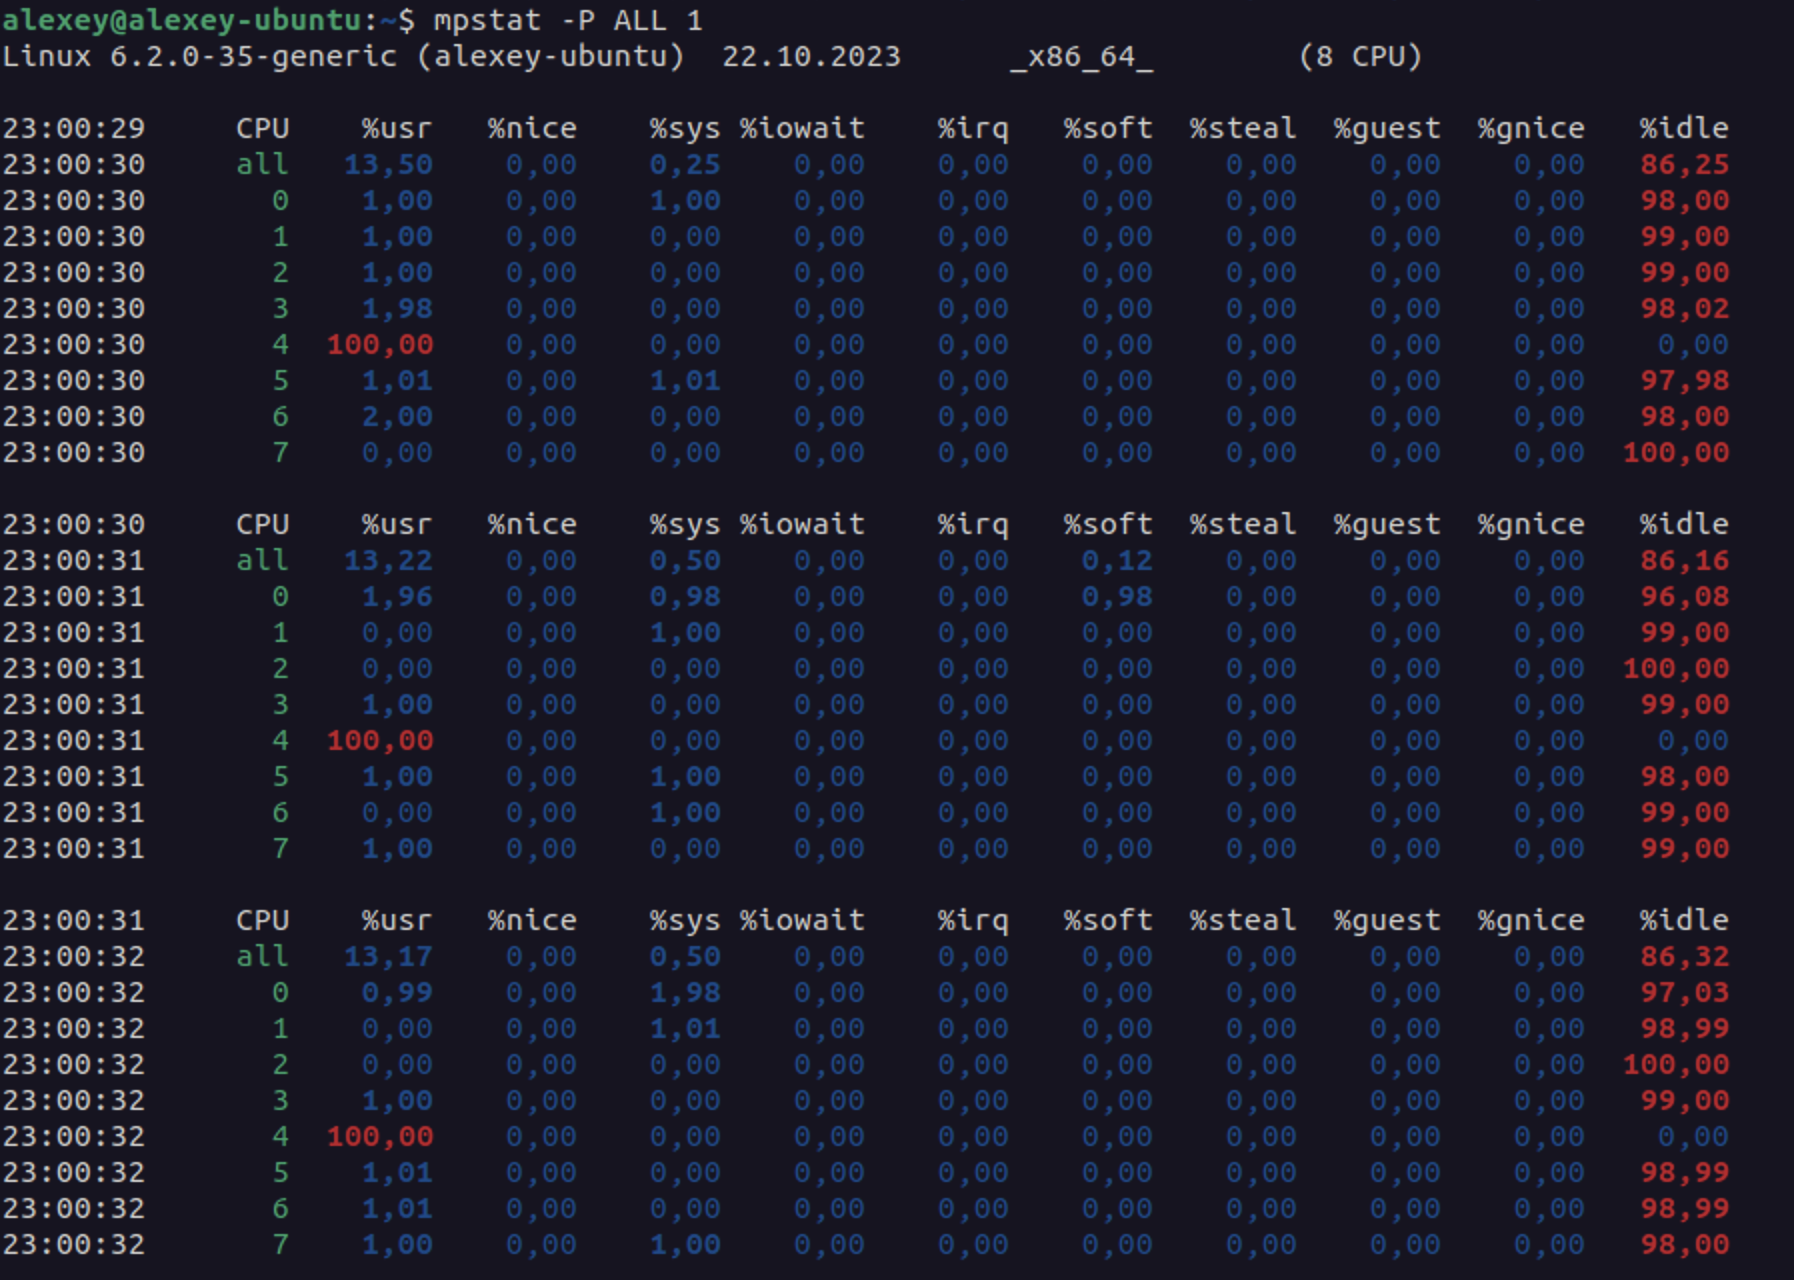
\includegraphics[width=\textwidth]{image/mpstat.png}
Видим, что \textit{stress-ng} загружает только один процессор на 100\% (в данном случае процессор 4).
Такое поведение и ожидалось так как мы запустили \textit{stress-ng} с параматром \textit{--cpu 1}.
Для следующих запусков определим командой \textit{taskset} процессор на котором будет выполняться \textit{stress-ng}.\\
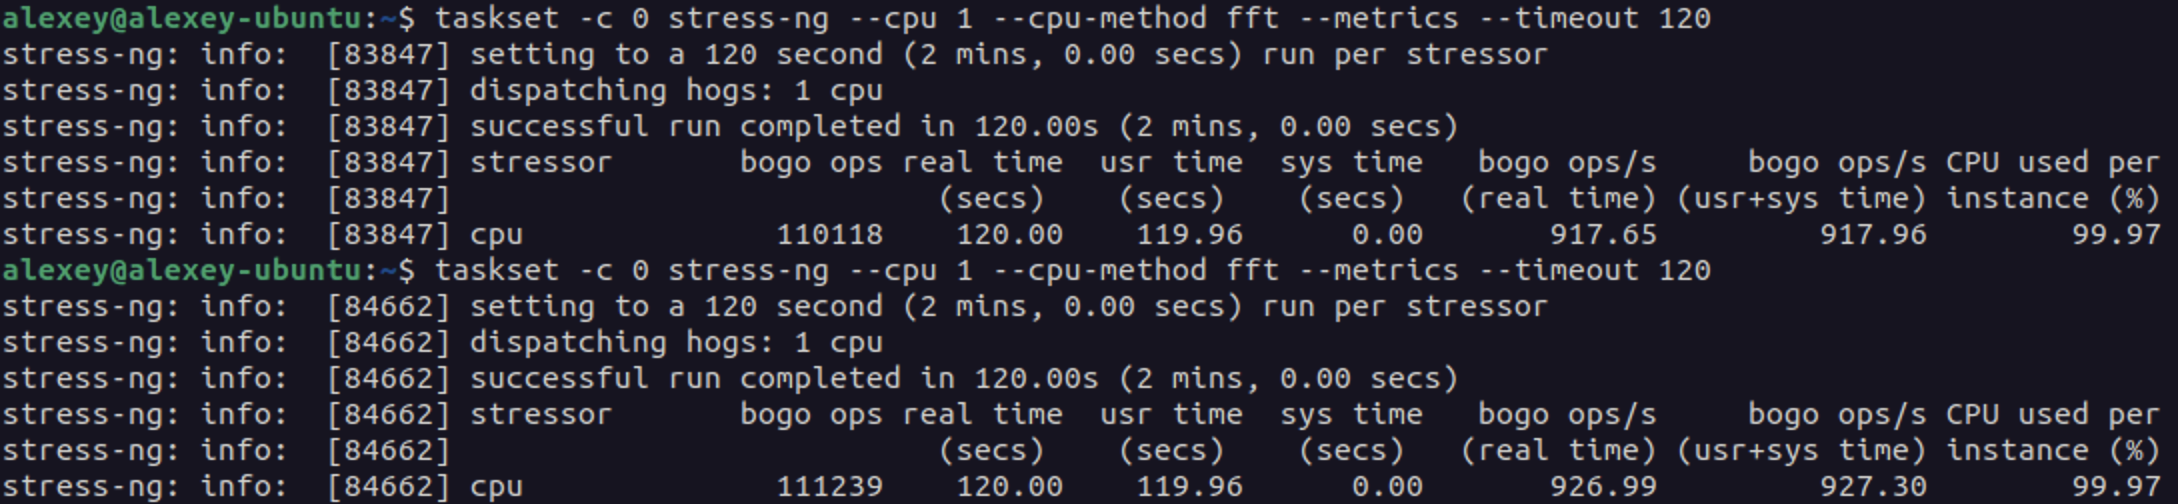
\includegraphics[width=\textwidth]{image/taskset.png}
Как мы можем заметить, производительность немного подросла, особенно это видно при повторном запуске. Это следует из того, что при использовании одного и того же процессора кеши остаются горячими.\\ 
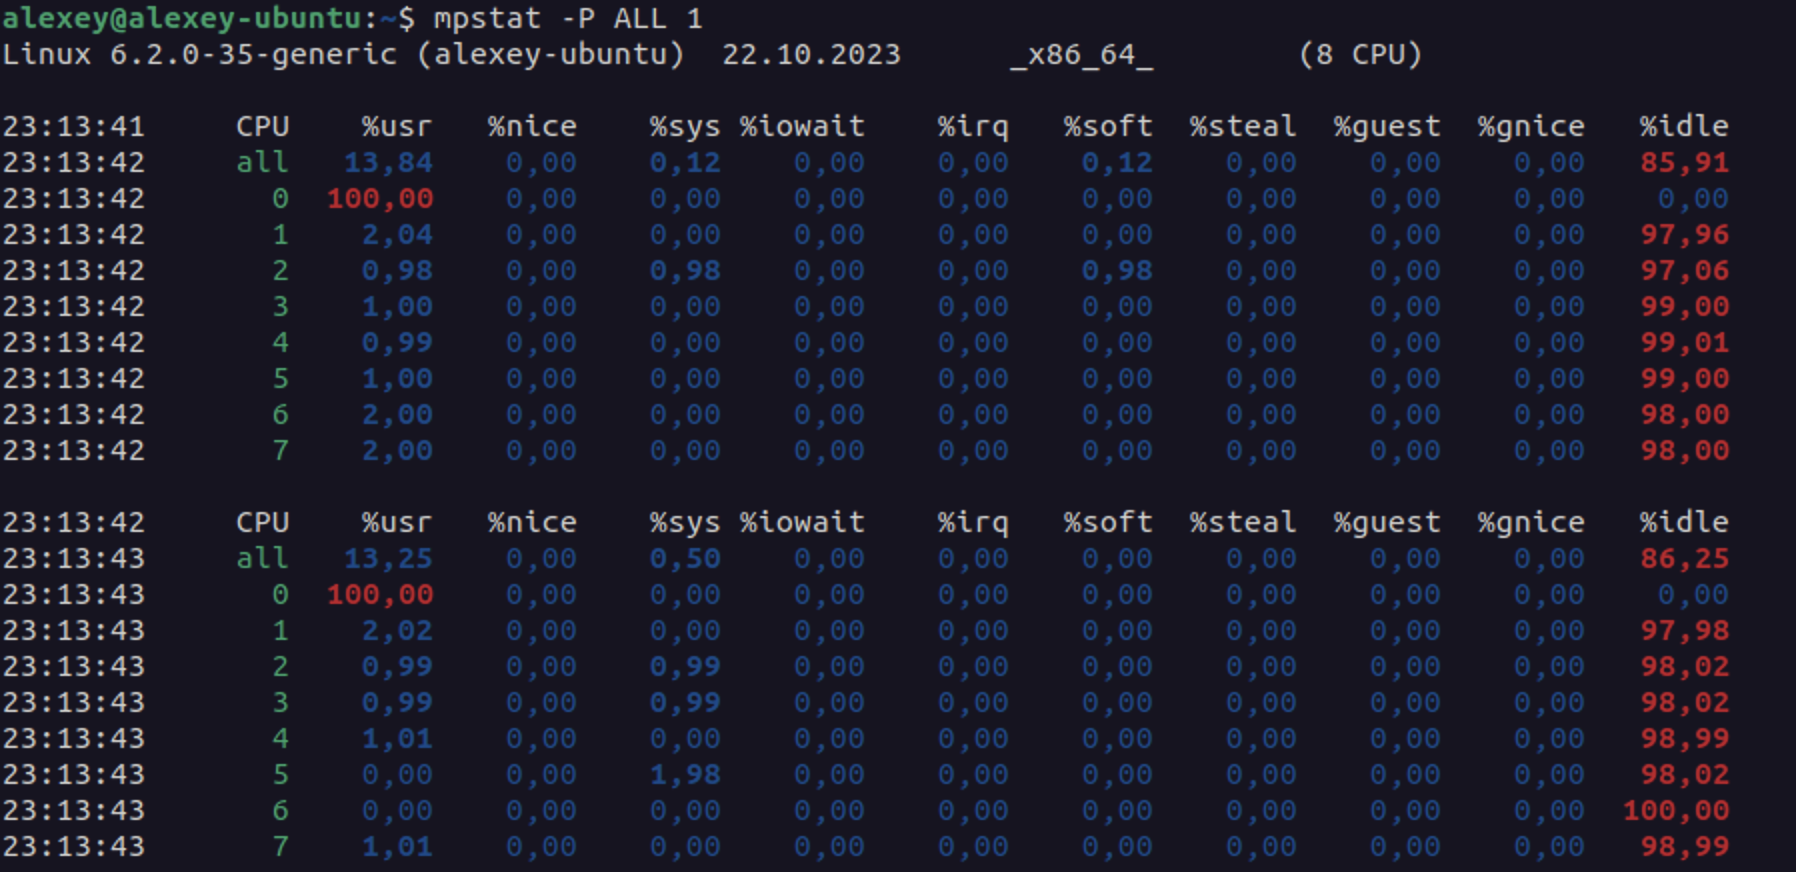
\includegraphics[width=\textwidth]{image/mpstat2.png}
\subsubsection{Команда atop}
С помощью команды \textit{atop}, которая является более специфичным для Linux аналогом команды top, мы посмотрим общую загруженность системы.\\
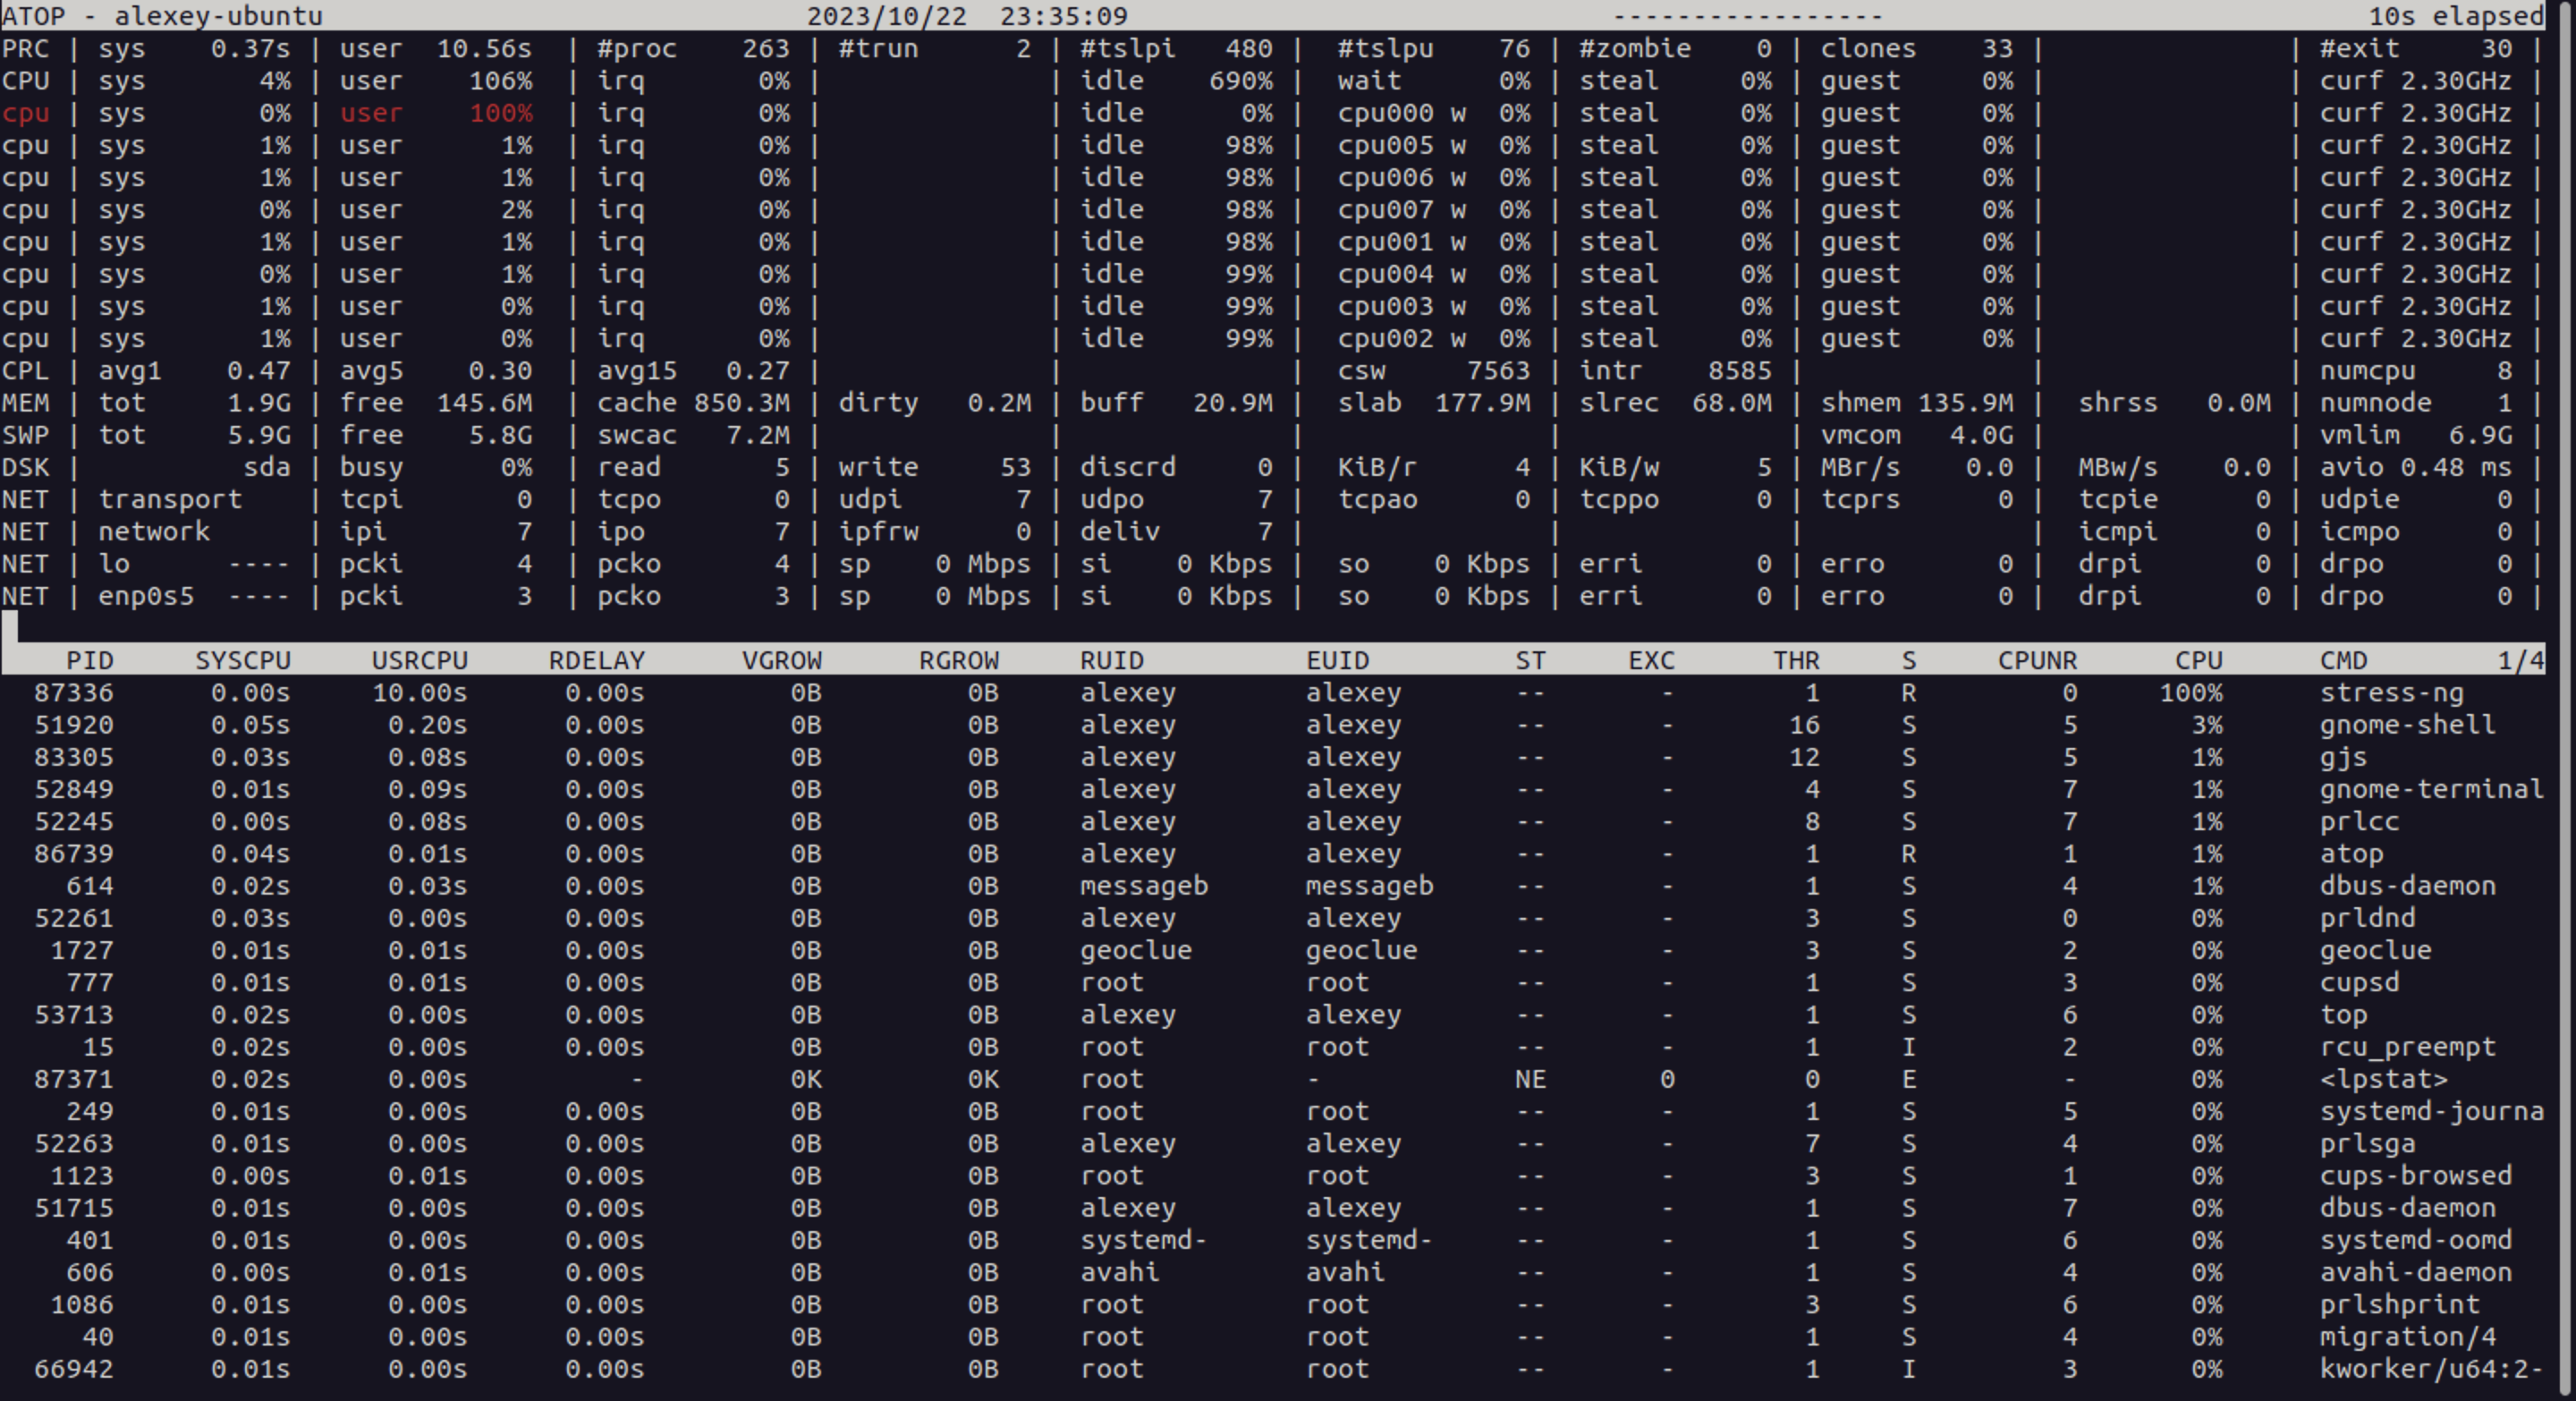
\includegraphics[width=\textwidth]{image/atop2.png}
Отсюда мы делаем вывод, что кроме нашего процесса самое высокое потребление у \textit{gnome-shell}, но пока мы рассматриваем нагрузку только на одно ядро для нас это неважно, потому что gnome-shell будет выполняться на другом ядре.\\
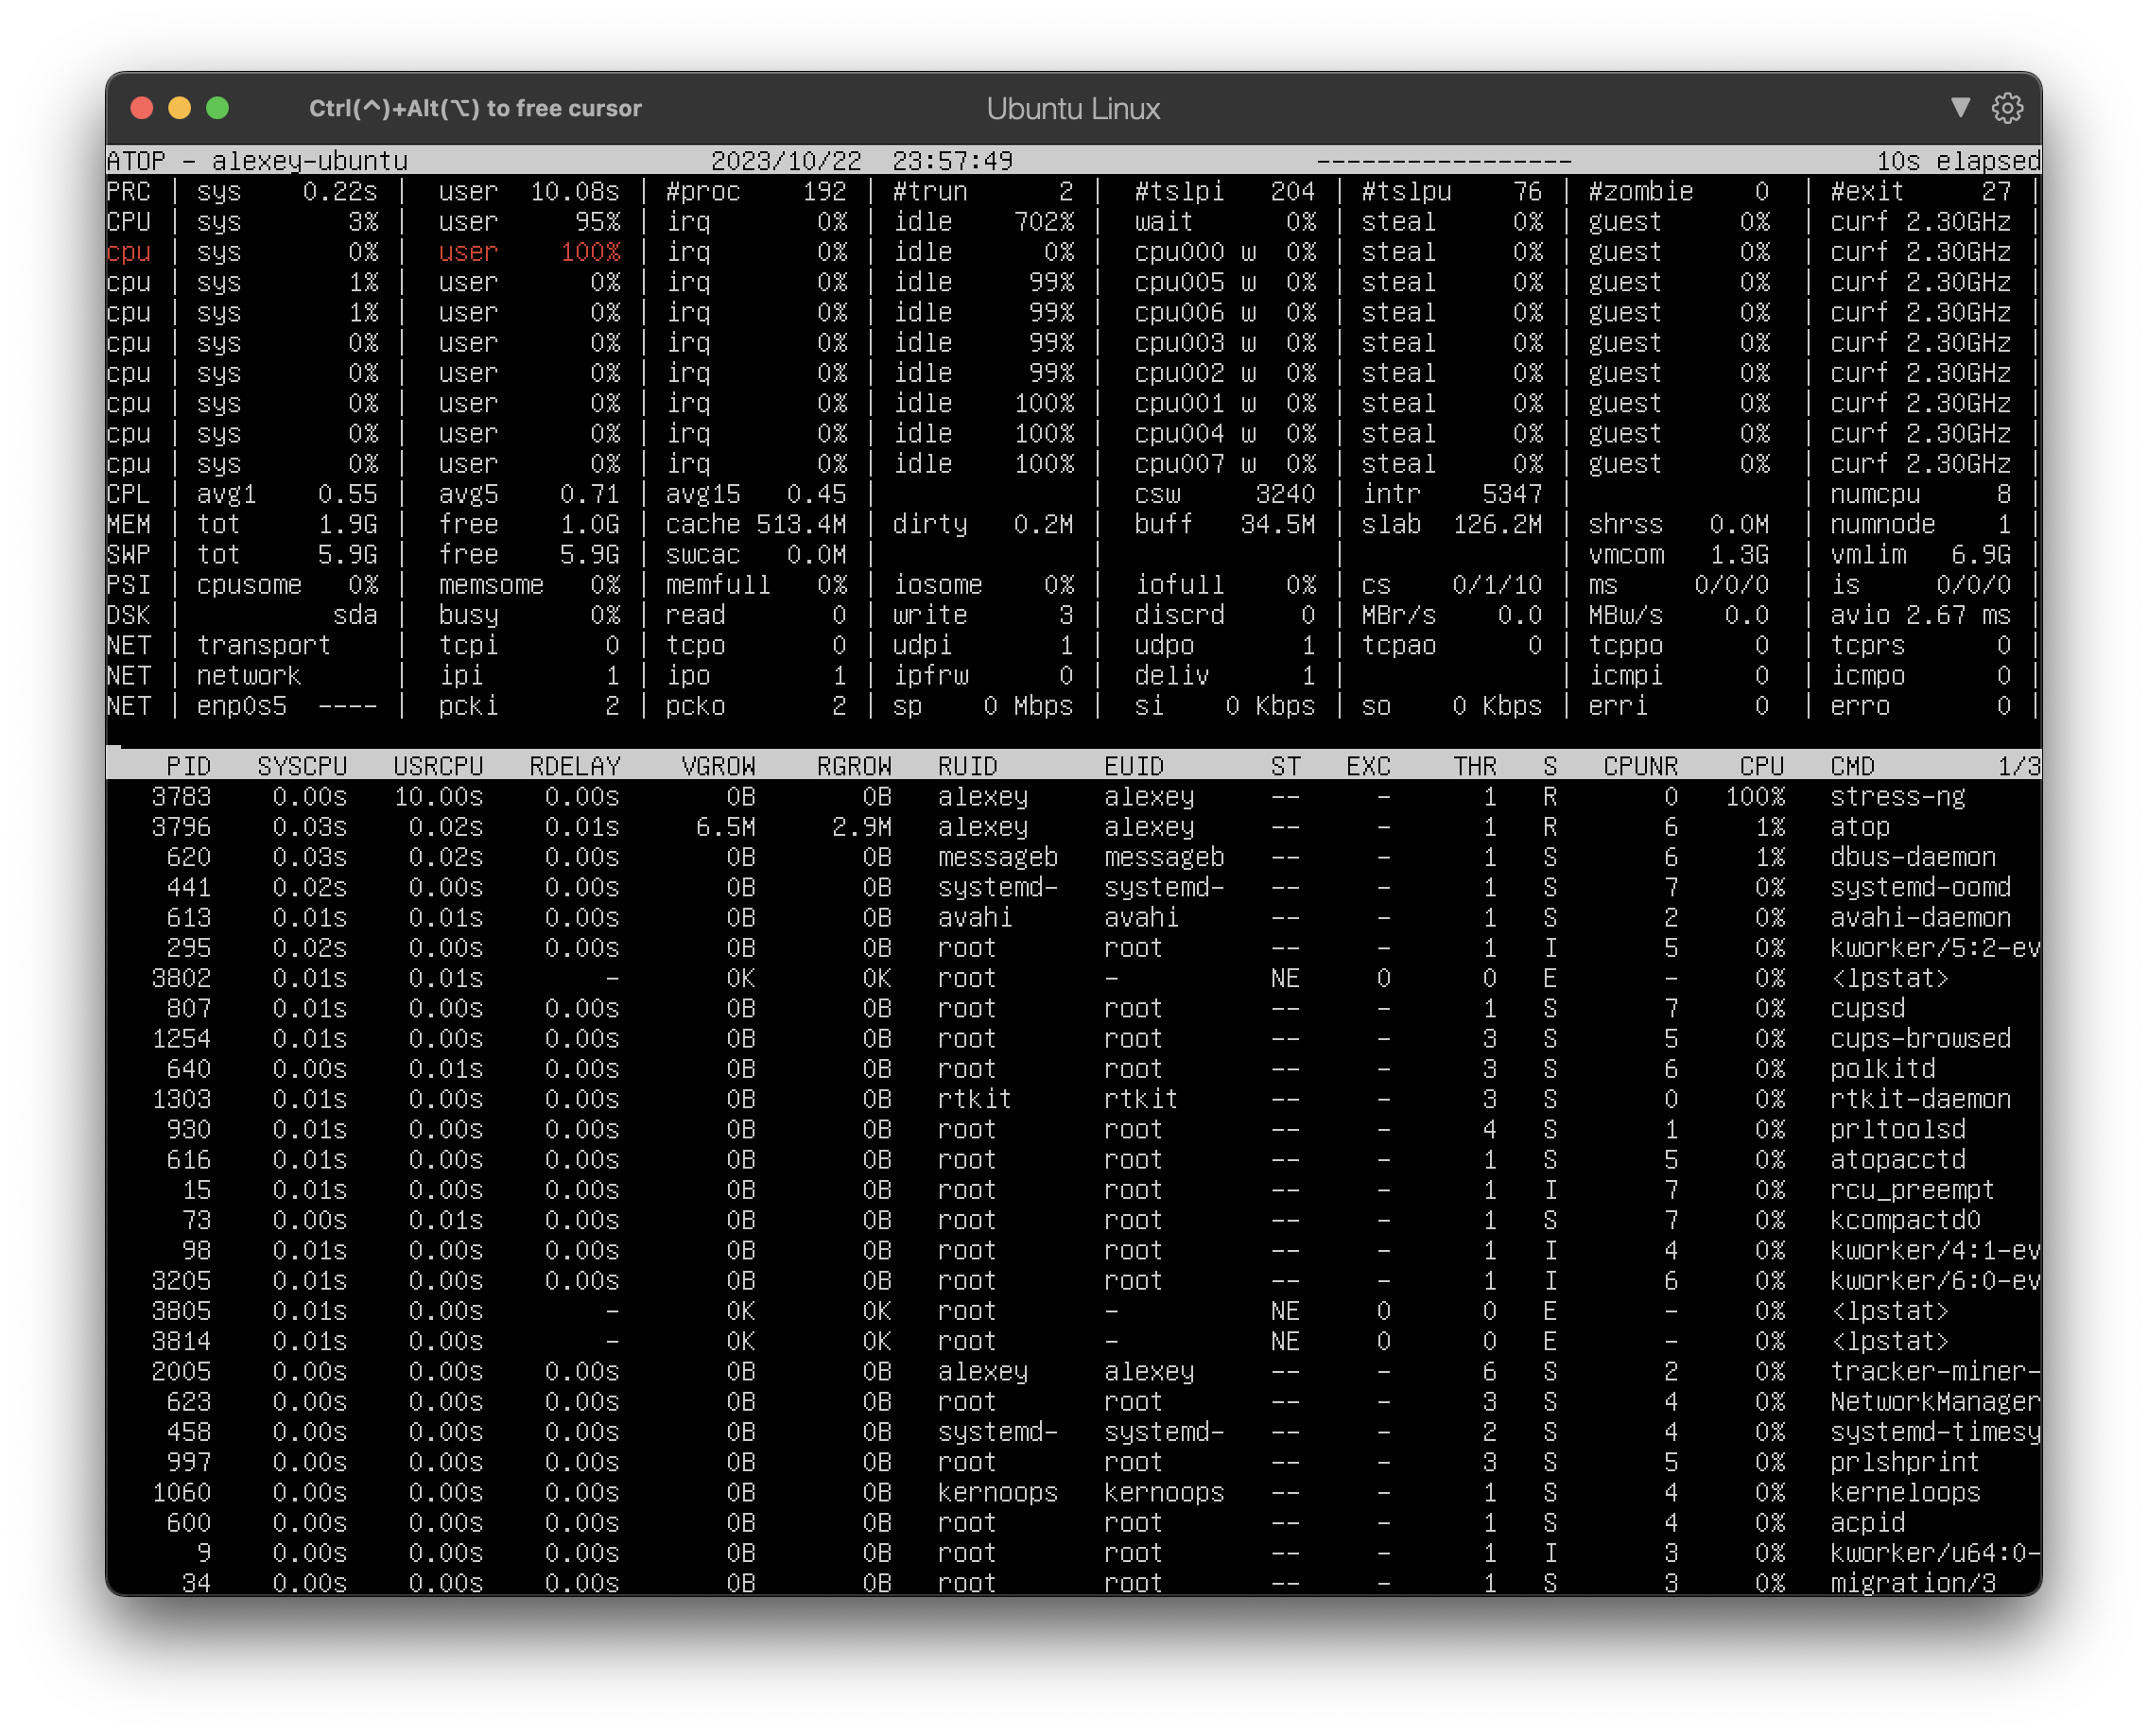
\includegraphics[width=\textwidth]{image/atop3.png}
Запустили без графической оболочки. \\
Как и ожидалось прироста производительности нет, пока мы рассматриваем тесты для одного ядра.\\
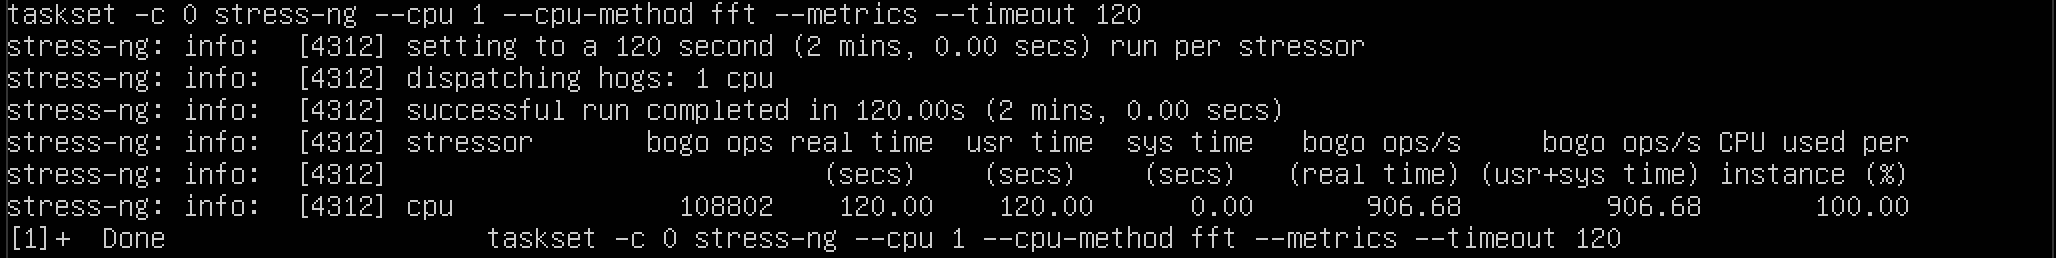
\includegraphics[width=\textwidth]{image/gnome.png}
\subsubsection{Команда stress-ng}
Воспользуемся встроенными параметрами \textit{stress-ng}.\\
С помощью опции --times можно получить представление о том, сколько пользовательского и системного (ядро) времени используется.\\
Мы можем запустить \textit{stress-ng} с опцией --perf, чтобы увидеть более подробную информацию о том, что делает машина во время работы\\
{\lstconsolestyle
\definecolor{xxxhtmlcolorIMAIMP}{HTML}{26A269}
\definecolor{xxxhtmlcolorHIKOOB}{HTML}{12488B}\begin{lstlisting}
%*{\color{xxxhtmlcolorIMAIMP}{\bfseries alexey@alexey{-}ubuntu}}*):%*{\color{xxxhtmlcolorHIKOOB}{\bfseries \textasciitilde{}}}*)$ taskset -c 0 sudo stress-ng --cpu 1 --cpu-method fft --metrics --timeout 120 --times --perf
[sudo] password for alexey: 
stress-ng: info:  [3347] setting to a 120 second (2 mins, 0.00 secs) run per stressor
stress-ng: info:  [3347] dispatching hogs: 1 cpu
stress-ng: info:  [3347] successful run completed in 121.46s (2 mins, 1.46 secs)
stress-ng: info:  [3347] stressor       bogo ops real time  usr time  sys time   bogo ops/s     bogo ops/s CPU used per
stress-ng: info:  [3347]                           (secs)    (secs)    (secs)   (real time) (usr+sys time) instance (%)
stress-ng: info:  [3347] cpu              109925    121.46    119.88      0.05       905.06         916.58        98.74
stress-ng: info:  [3347] cpu:
stress-ng: info:  [3347]      119 873 637 761 CPU Clock                       0.99 B/sec
stress-ng: info:  [3347]      119 867 619 227 Task Clock                      0.99 B/sec
stress-ng: info:  [3347]                         44 Page Faults Total               0,36 /sec 
stress-ng: info:  [3347]                         44 Page Faults Minor               0,36 /sec 
stress-ng: info:  [3347]                          0 Page Faults Major               0,00 /sec 
stress-ng: info:  [3347]                        763 Context Switches                6,28 /sec 
stress-ng: info:  [3347]                        761 Cgroup Switches                 6,27 /sec 
stress-ng: info:  [3347]                          0 CPU Migrations                  0,00 /sec 
stress-ng: info:  [3347]                          0 Alignment Faults                0,00 /sec 
stress-ng: info:  [3347]                          0 Emulation Faults                0,00 /sec 
stress-ng: info:  [3347]                         43 Page Faults User                0,35 /sec 
stress-ng: info:  [3347]                          1 Page Faults Kernel              0,01 /sec 
stress-ng: info:  [3347]                         92 System Call Enter               0,76 /sec 
stress-ng: info:  [3347]                         91 System Call Exit                0,75 /sec 
stress-ng: info:  [3347]                          1 Kmalloc                         0,01 /sec 
stress-ng: info:  [3347]                          1 Kfree                           0,01 /sec 
stress-ng: info:  [3347]                          3 Kmem Cache Alloc                0,02 /sec 
stress-ng: info:  [3347]                          2 Kmem Cache Free                 0,02 /sec 
stress-ng: info:  [3347]                         35 MM Page Alloc                   0,29 /sec 
stress-ng: info:  [3347]                          0 MM Page Free                    0,00 /sec 
stress-ng: info:  [3347]                   79.202 RCU Utilization               652.10 /sec 
stress-ng: info:  [3347]                          9 Sched Migrate Task              0,07 /sec 
stress-ng: info:  [3347]                          0 Sched Move NUMA                 0,00 /sec 
stress-ng: info:  [3347]                        765 Sched Wakeup                    6,30 /sec 
stress-ng: info:  [3347]                          0 Sched Proc Exec                 0,00 /sec 
stress-ng: info:  [3347]                          0 Sched Proc Exit                 0,00 /sec 
stress-ng: info:  [3347]                          0 Sched Proc Fork                 0,00 /sec 
stress-ng: info:  [3347]                          0 Sched Proc Free                 0,00 /sec 
stress-ng: info:  [3347]                          0 Sched Proc Hang                 0,00 /sec 
stress-ng: info:  [3347]                          0 Sched Proc Wait                 0,00 /sec 
stress-ng: info:  [3347]                        763 Sched Switch                    6,28 /sec 
stress-ng: info:  [3347]                          2 Signal Generate                 0,02 /sec 
stress-ng: info:  [3347]                          1 Signal Deliver                  0,01 /sec 
stress-ng: info:  [3347]                         32 IRQ Entry                       0,26 /sec 
stress-ng: info:  [3347]                         32 IRQ Exit                        0,26 /sec 
stress-ng: info:  [3347]                   11.185 Soft IRQ Entry                 92.09 /sec 
stress-ng: info:  [3347]                   11.185 Soft IRQ Exit                  92.09 /sec 
stress-ng: info:  [3347]                          0 NMI handler                     0,00 /sec 
stress-ng: info:  [3347]                          1 Writeback Dirty Inode           0,01 /sec 
stress-ng: info:  [3347]                          0 Migrate MM Pages                0,00 /sec 
stress-ng: info:  [3347]                          1 SKB Consume                     0,01 /sec 
stress-ng: info:  [3347]                          0 SKB Kfree                       0,00 /sec 
stress-ng: info:  [3347]                          0 IOMMU IO Page Fault             0,00 /sec 
stress-ng: info:  [3347]                          0 IOMMU Map                       0,00 /sec 
stress-ng: info:  [3347]                          0 IOMMU Unmap                     0,00 /sec 
stress-ng: info:  [3347]                          0 Filemap page-cache add          0,00 /sec 
stress-ng: info:  [3347]                          0 Filemap page-cache del          0,00 /sec 
stress-ng: info:  [3347]                          0 OOM Compact Retry               0,00 /sec 
stress-ng: info:  [3347]                          0 OOM Wake Reaper                 0,00 /sec 
stress-ng: info:  [3347]                          0 Thermal Zone Trip               0,00 /sec 
stress-ng: info:  [3347] for a 121,46s run time:
stress-ng: info:  [3347]     971,66s available CPU time
stress-ng: info:  [3347]     119,88s user time   ( 12,34%)
stress-ng: info:  [3347]       0,05s system time (  0,01%)
stress-ng: info:  [3347]     119,93s total time  ( 12,34%)
stress-ng: info:  [3347] load average: 1,09 0,69 0,30
\end{lstlisting}}
\subsubsection{Flame Graph}
Выполняем профилирование в течении 10 секунд.\\
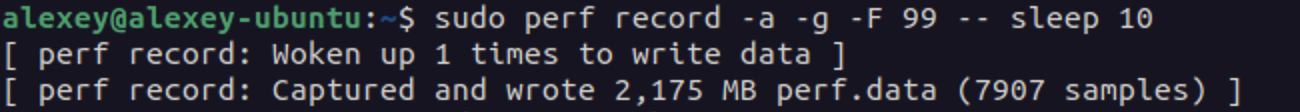
\includegraphics[width=\textwidth]{image/perf.png}
Строим по выводу Flame Graph.\\
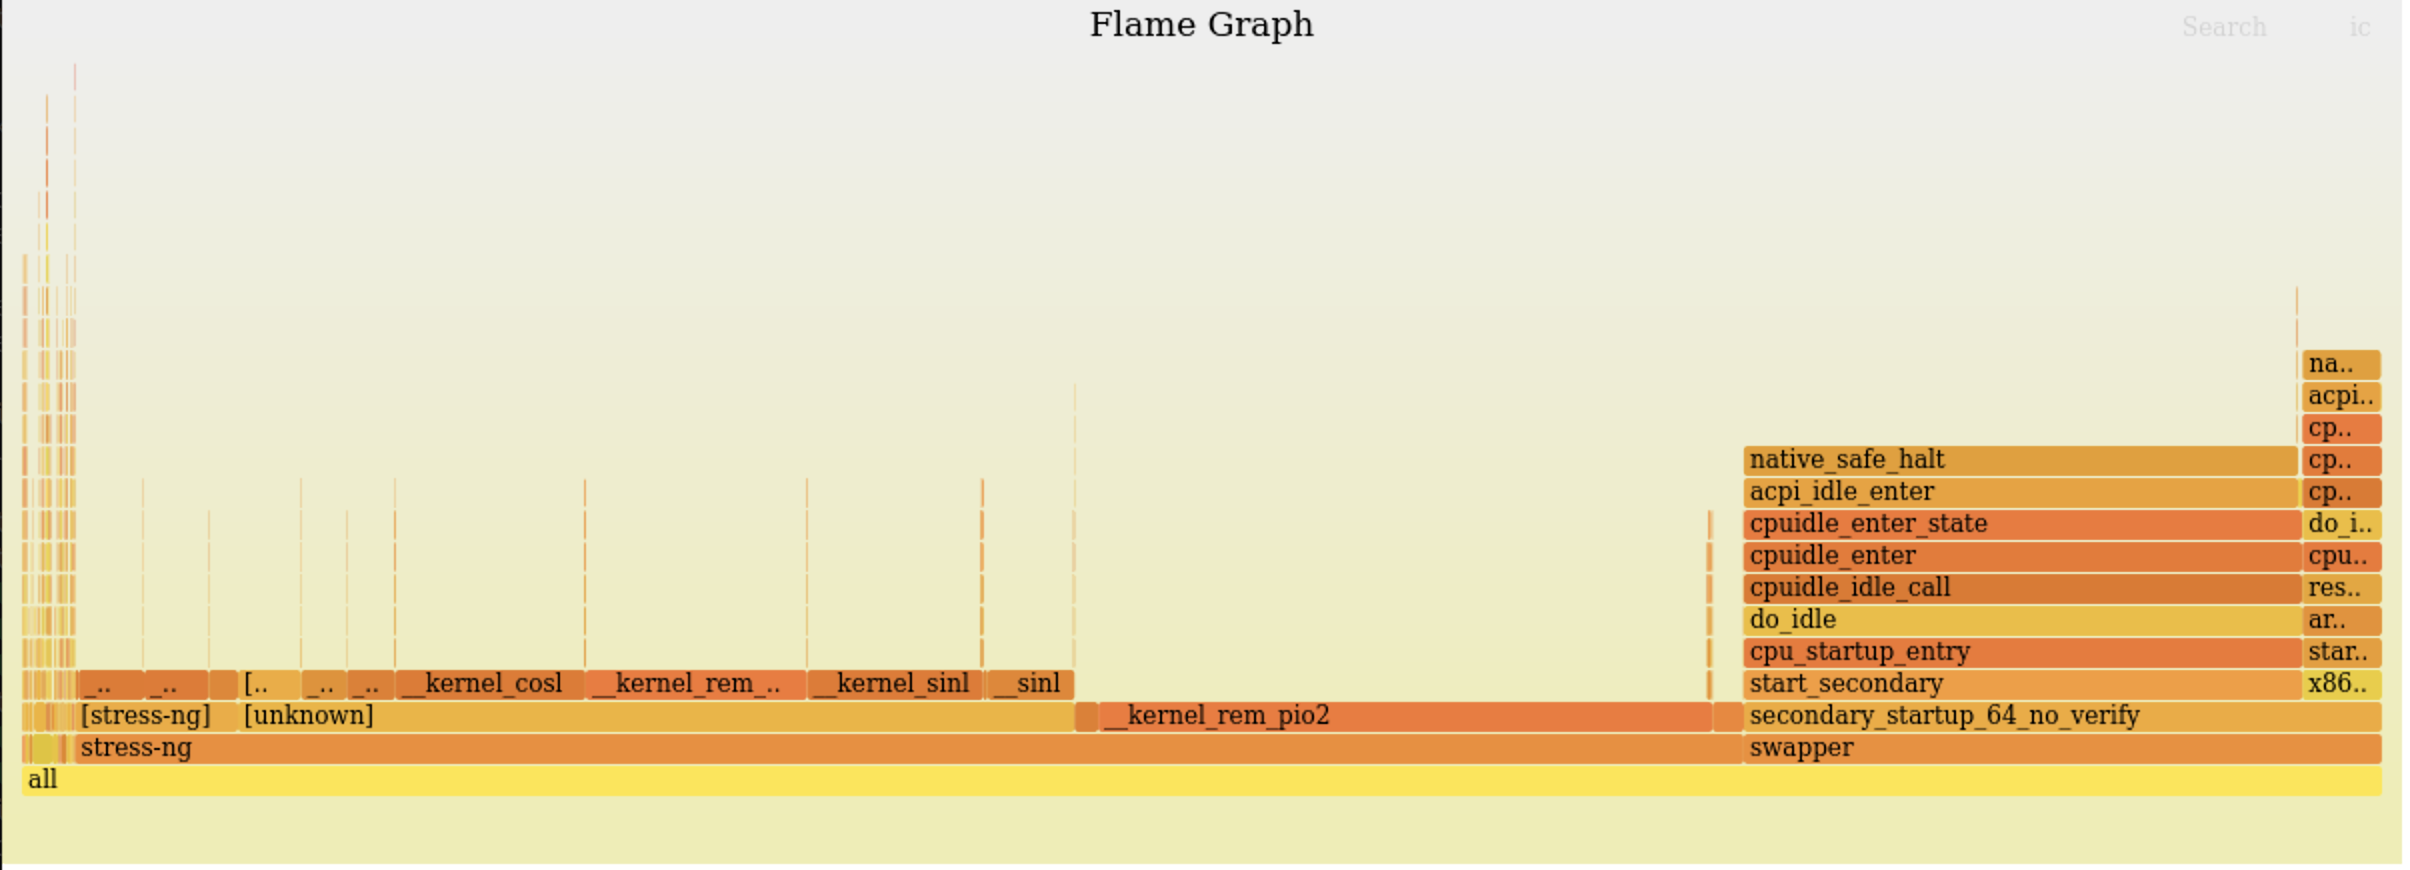
\includegraphics[width=\textwidth]{image/flamegraph.png}
\subsection{Переходим к активным действиям}
\subsubsection{Команда nice}
Повысим приоритет нашего процесса с помощью команды \textit{nice}.\\
Чтобы была конкуренция за ресурс процессора, мы запустим тест на все ядра (8 ядер)\\
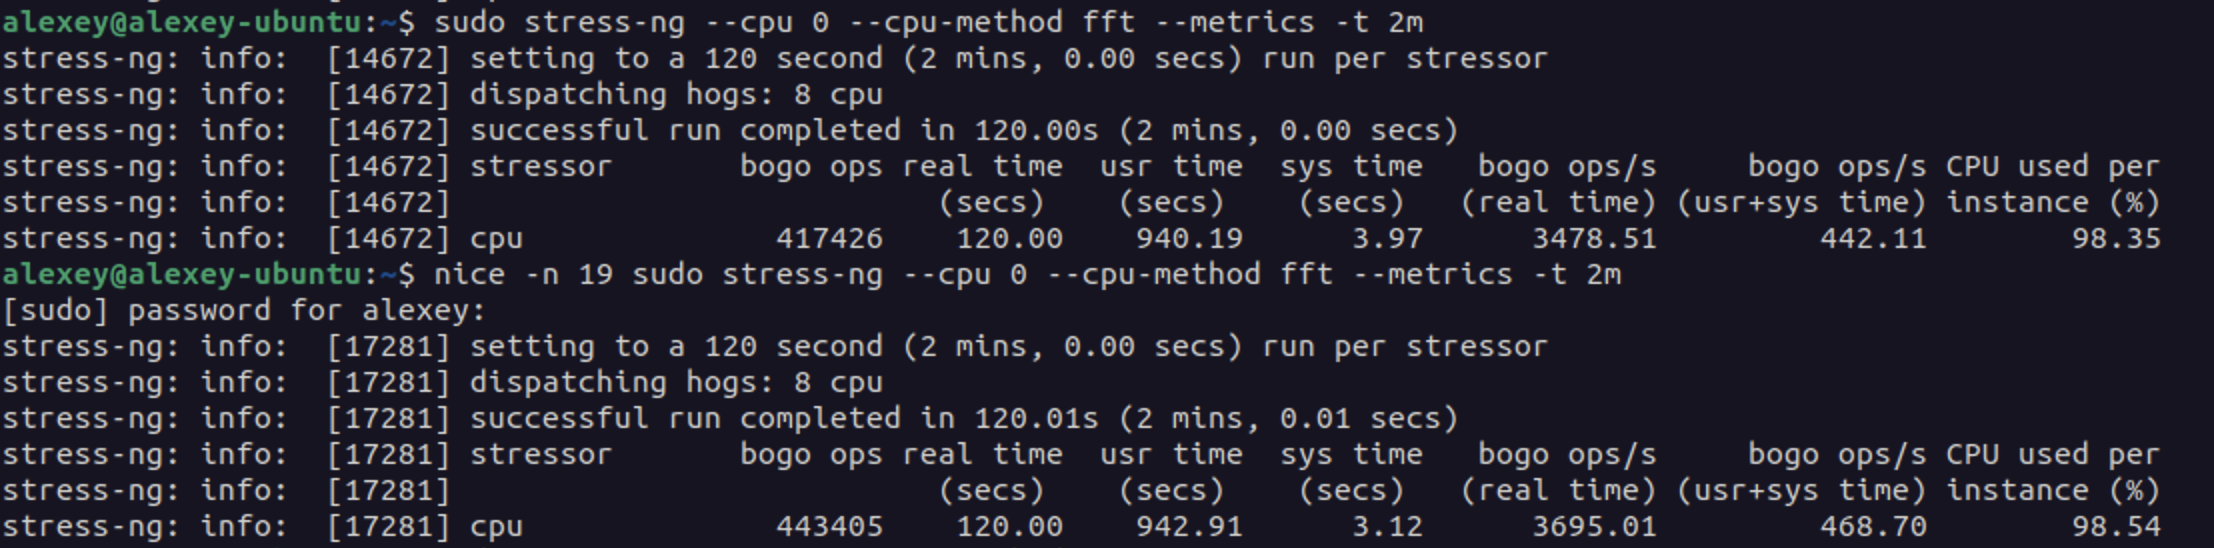
\includegraphics[width=\textwidth]{image/nice.png}
Видим, что с увеличением приоритета мы немного выиграли в производительности.
\subsubsection{Команда chrt}
Попробуем разные политики планирования для наших процессов.\\
\nquote{RR (Round Robin)}{SCHED\_RR — это алгоритм планирования циклическим перебором. Как только поток исчерпает свой квант времени, он перемещается в конец очереди на выполнение для своего уровня приоритета. Это позволяет запускать другие потоки с таким же приоритетом. Использует класс планирования RT.}
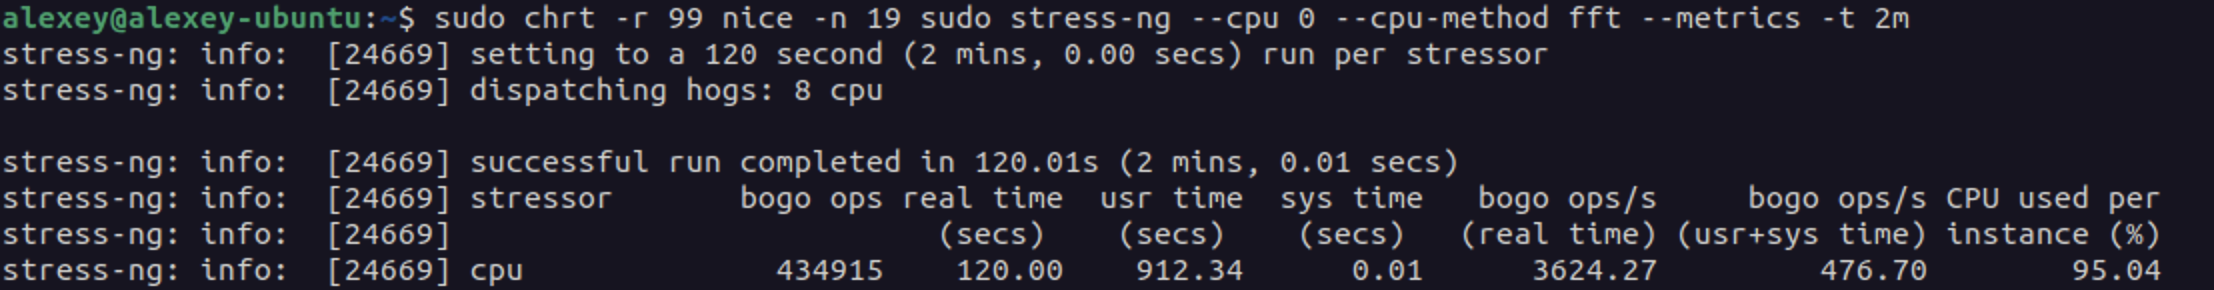
\includegraphics[width=\textwidth]{image/rr.png}
\nquote{FIFO (First In, First Out)}{SCHED\_FIFO — это алгоритм планирования «первым пришел, первым вышел», который продолжает выполнять поток, находящийся в голове очереди на выполнение, пока тот не оставит процессор добровольно или не появится поток с более высоким приоритетом. Поток продолжает выполняться, даже если в очереди на выполнение есть другие потоки с таким же приоритетом. Использует класс планирования RT.}
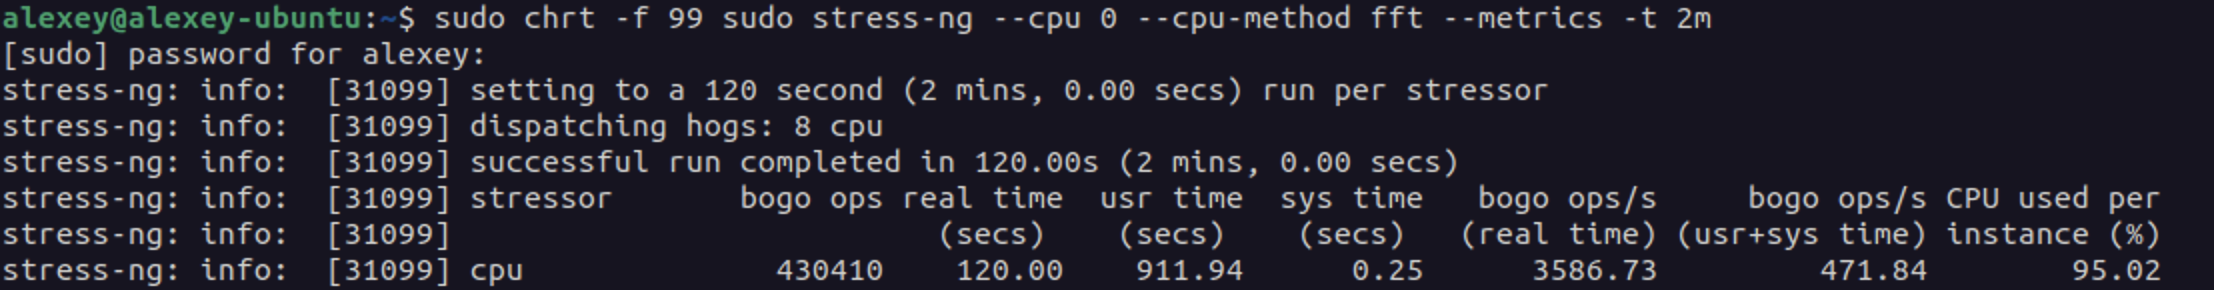
\includegraphics[width=\textwidth]{image/fifo.png}
\nquote{NORMAL}{SCHED\_NORMAL (ранее известный как SCHED\_OTHER) — это алгоритм планирования с разделением времени. Используется по умолчанию для пользовательских процессов. Планировщик динамически корректирует приоритет в зависимости от класса планирования. Для O(1) длительность кванта времени устанавливается на основе статического приоритета: чем выше приоритет, тем больше квант времени. Для класса CFS размер кванта выбирается динамически. Использует класс планирования CFS.}
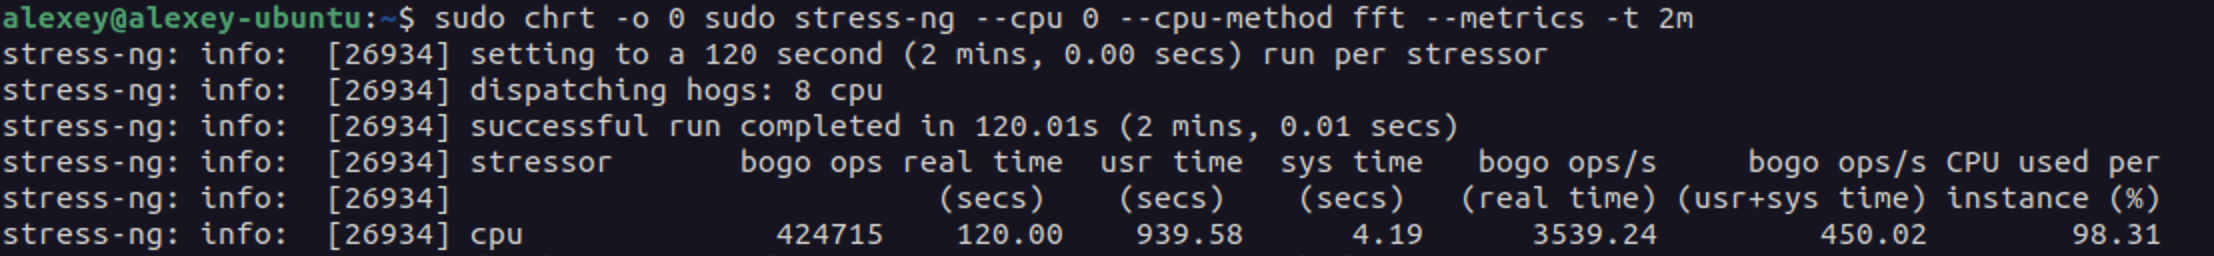
\includegraphics[width=\textwidth]{image/normal.png}
\nquote{BATCH}{SCHED\_BATCH — этот алгоритм действует как SCHED\_NORMAL, но ожидается, что поток будет привязан к процессору и не должен прерывать другие интерактивные задачи, связанные с вводом/выводом. Использует класс планирования CFS.}
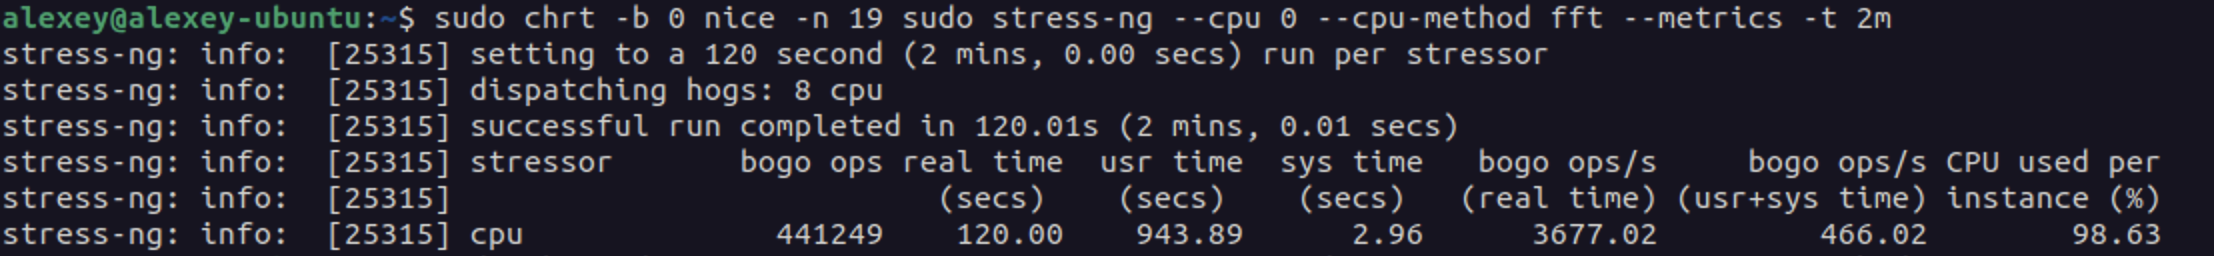
\includegraphics[width=\textwidth]{image/batch.png}
\nquote{IDLE:}{SCHED\_IDLE использует класс планирования Idle.}
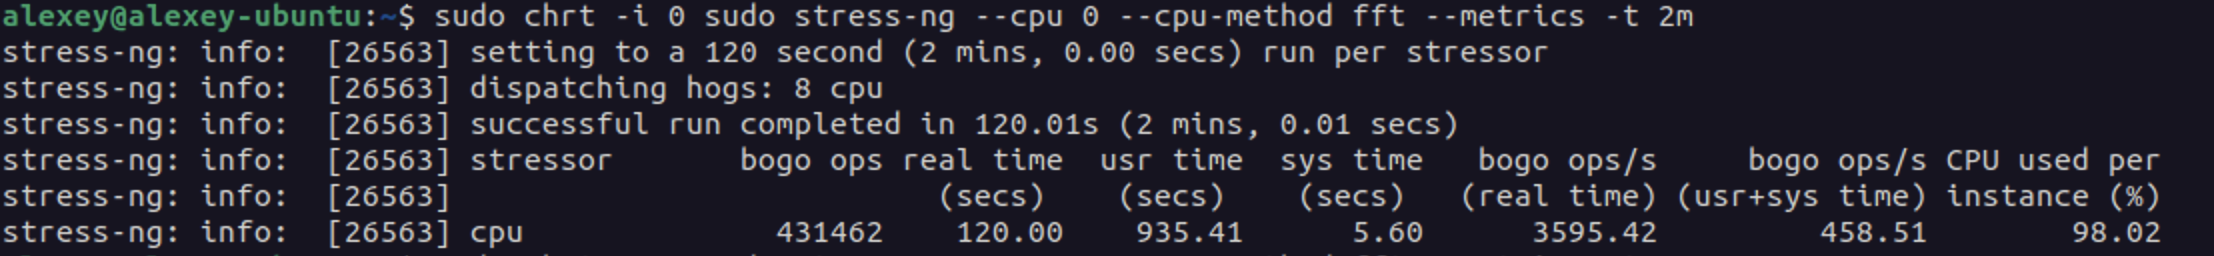
\includegraphics[width=\textwidth]{image/idle.png}
Как мы видим, выбор политики планирования не сильно влияет на производительность нашего теста.
\subsubsection{Финал}
Отключаем графический интерфейс и применяем все настройки выше. \\
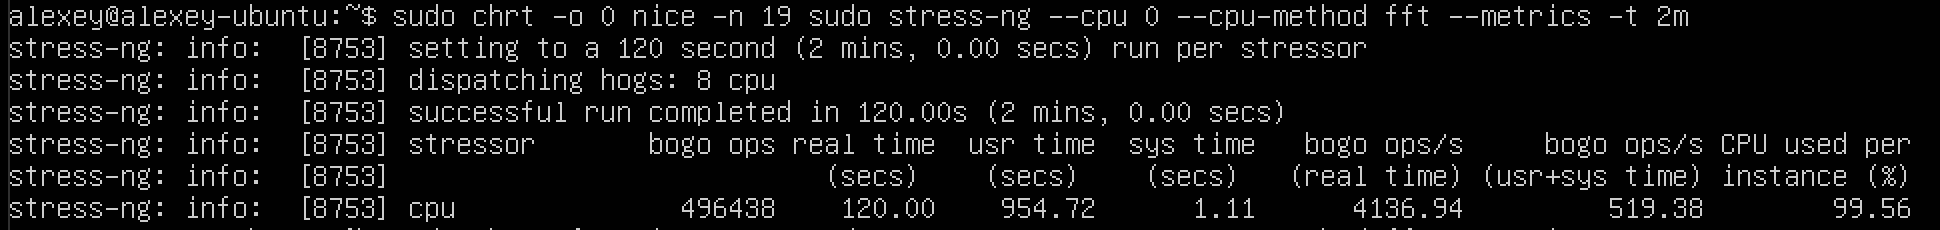
\includegraphics[width=\textwidth]{image/cpu-max.png}
Итого мы с \textbf{417426} bogo ops смогли повысить проиизводительность до \textbf{496438} bogo ops.
\subsection{cdouble}
Так как \textit{cdouble} тоже вычислительная задача, то попробуем применить все настройки выше.\\
Но сначала тест без настроек. \\
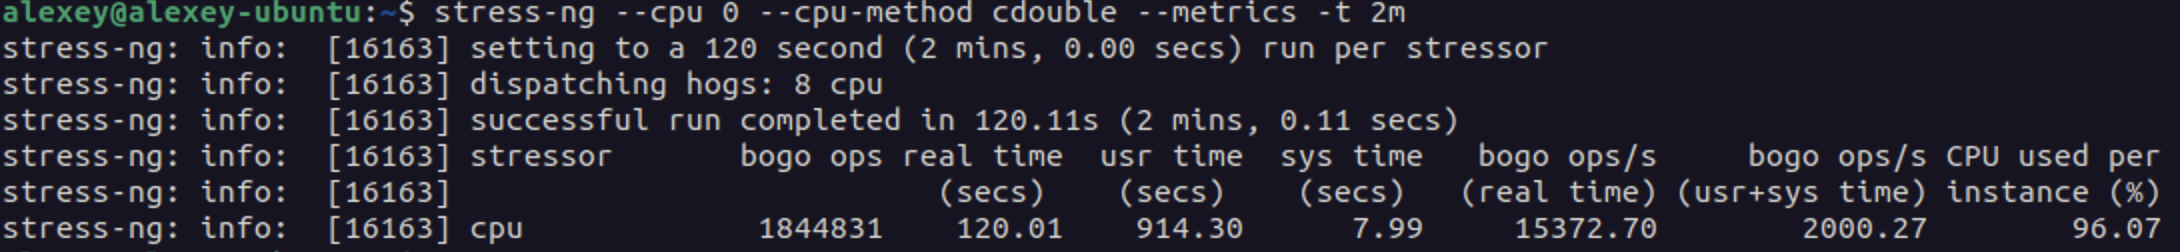
\includegraphics[width=\textwidth]{image/cdouble-1.png}
Посмотрим потребление процессора.\\
\begin{verbatim}
14:39:30      UID       PID    %usr %system  %guest   %wait    %CPU   CPU  Command
14:39:31     1000     16167   96,00    1,00    0,00    4,00   97,00     0  stress-ng
14:39:32     1000     16167   99,01    0,00    0,00    0,99   99,01     0  stress-ng
14:39:33     1000     16167  100,00    0,00    0,00    0,00  100,00     0  stress-ng
14:39:34     1000     16167   96,00    0,00    0,00    2,00   96,00     0  stress-ng
14:39:35     1000     16167   96,00    1,00    0,00    4,00   97,00     0  stress-ng
14:39:36     1000     16167   97,00    1,00    0,00    3,00   98,00     0  stress-ng
14:39:37     1000     16167   95,00    0,00    0,00    4,00   95,00     0  stress-ng
14:39:38     1000     16167   99,00    1,00    0,00    1,00  100,00     0  stress-ng
14:39:39     1000     16167   95,00    1,00    0,00    4,00   96,00     5  stress-ng
14:39:40     1000     16167   95,00    0,00    0,00    5,00   95,00     5  stress-ng
14:39:41     1000     16167   97,00    0,00    0,00    3,00   97,00     5  stress-ng
14:39:42     1000     16167   96,00    0,00    0,00    3,00   96,00     5  stress-ng
14:39:43     1000     16167   97,00    1,00    0,00    3,00   98,00     5  stress-ng
14:39:44     1000     16167   96,00    1,00    0,00    3,00   97,00     5  stress-ng
14:39:45     1000     16167   95,00    1,00    0,00    4,00   96,00     5  stress-ng
14:39:46     1000     16167   93,00    1,00    0,00    6,00   94,00     5  stress-ng
14:39:47     1000     16167   95,05    0,99    0,00    2,97   96,04     5  stress-ng
14:39:48     1000     16167   98,00    0,00    0,00    3,00   98,00     5  stress-ng
14:39:49     1000     16167   95,05    1,98    0,00    1,98   97,03     5  stress-ng
14:39:50     1000     16167   95,00    2,00    0,00    3,00   97,00     3  stress-ng
14:39:51     1000     16167   97,00    0,00    0,00    3,00   97,00     3  stress-ng
14:39:52     1000     16167   95,05    0,99    0,00    3,96   96,04     3  stress-ng
14:39:53     1000     16167   96,00    0,00    0,00    3,00   96,00     3  stress-ng
14:39:54     1000     16167   97,00    1,00    0,00    4,00   98,00     3  stress-ng
14:39:55     1000     16167   95,00    0,00    0,00    3,00   95,00     3  stress-ng
14:39:56     1000     16167   95,00    2,00    0,00    5,00   97,00     3  stress-ng
14:39:57     1000     16167   92,00    3,00    0,00    5,00   95,00     3  stress-ng
14:39:58     1000     16167  100,00    0,00    0,00    0,00  100,00     3  stress-ng
14:39:59     1000     16167   93,00    0,00    0,00    7,00   93,00     3  stress-ng
14:40:00     1000     16167   96,00    0,00    0,00    3,00   96,00     3  stress-ng
14:40:01     1000     16167   92,08    0,00    0,00    6,93   92,08     3  stress-ng
14:40:02     1000     16167   94,00    2,00    0,00    6,00   96,00     3  stress-ng
14:40:03     1000     16167   91,00    1,00    0,00    8,00   92,00     3  stress-ng
14:40:04     1000     16167   93,00    0,00    0,00    6,00   93,00     3  stress-ng
14:40:05     1000     16167   99,00    1,00    0,00    1,00  100,00     3  stress-ng
14:40:06     1000     16167   96,00    0,00    0,00    4,00   96,00     3  stress-ng
14:40:07     1000     16167   96,04    0,00    0,00    2,97   96,04     3  stress-ng
14:40:08     1000     16167   97,00    1,00    0,00    1,00   98,00     3  stress-ng
14:40:09     1000     16167   98,00    1,00    0,00    2,00   99,00     3  stress-ng
14:40:10     1000     16167   98,00    0,00    0,00    2,00   98,00     3  stress-ng
14:40:11     1000     16167   93,00    3,00    0,00    5,00   96,00     3  stress-ng

14:40:11      UID       PID    %usr %system  %guest   %wait    %CPU   CPU  Command
14:40:12     1000     16167  100,00    0,00    0,00    0,00  100,00     3  stress-ng
14:40:13     1000     16167   99,00    0,00    0,00    1,00   99,00     3  stress-ng
14:40:14     1000     16167   97,03    0,99    0,00    1,98   98,02     3  stress-ng
14:40:15     1000     16167   92,08    0,99    0,00    5,94   93,07     3  stress-ng
14:40:16     1000     16167   99,00    0,00    0,00    2,00   99,00     3  stress-ng
14:40:17     1000     16167   99,00    0,00    0,00    1,00   99,00     5  stress-ng
14:40:18     1000     16167   91,00    1,00    0,00    9,00   92,00     5  stress-ng
14:40:19     1000     16167   92,00    0,00    0,00    6,00   92,00     5  stress-ng
14:40:20     1000     16167   96,04    0,00    0,00    3,96   96,04     5  stress-ng
14:40:21     1000     16167   96,00    0,00    0,00    4,00   96,00     5  stress-ng
14:40:22     1000     16167   99,00    0,00    0,00    2,00   99,00     5  stress-ng
14:40:23     1000     16167   96,00    0,00    0,00    4,00   96,00     5  stress-ng
14:40:24     1000     16167   93,00    1,00    0,00    6,00   94,00     5  stress-ng
14:40:25     1000     16167   88,24    2,94    0,00    9,80   91,18     5  stress-ng
14:40:26     1000     16167   93,88    1,02    0,00    5,10   94,90     5  stress-ng
14:40:27     1000     16167   93,00    1,00    0,00    5,00   94,00     5  stress-ng
14:40:28     1000     16167   93,14    0,00    0,00    5,88   93,14     5  stress-ng
14:40:29     1000     16167   99,00    0,00    0,00    1,00   99,00     5  stress-ng
14:40:30     1000     16167   97,03    0,00    0,00    2,97   97,03     5  stress-ng
14:40:31     1000     16167   97,00    1,00    0,00    2,00   98,00     5  stress-ng
14:40:32     1000     16167   97,00    2,00    0,00    2,00   99,00     5  stress-ng
14:40:33     1000     16167   95,00    0,00    0,00    5,00   95,00     5  stress-ng
14:40:34     1000     16167   93,00    3,00    0,00    4,00   96,00     5  stress-ng
14:40:35     1000     16167   95,00    0,00    0,00    5,00   95,00     5  stress-ng
14:40:36     1000     16167   95,00    0,00    0,00    5,00   95,00     5  stress-ng
14:40:37     1000     16167   95,00    1,00    0,00    4,00   96,00     5  stress-ng
14:40:38     1000     16167   91,00    2,00    0,00    7,00   93,00     5  stress-ng
14:40:39     1000     16167   98,00    0,00    0,00    2,00   98,00     5  stress-ng
14:40:40     1000     16167   93,00    3,00    0,00    4,00   96,00     5  stress-ng
14:40:41     1000     16167   96,00    2,00    0,00    1,00   98,00     5  stress-ng
14:40:42     1000     16167   97,09    0,00    0,00    2,91   97,09     0  stress-ng
14:40:43     1000     16167   97,00    1,00    0,00    3,00   98,00     0  stress-ng
14:40:44     1000     16167   94,00    0,00    0,00    6,00   94,00     0  stress-ng
14:40:45     1000     16167   95,00    0,00    0,00    0,00   95,00     0  stress-ng
14:40:46     1000     16167   96,00    4,00    0,00    5,00  100,00     0  stress-ng
14:40:47     1000     16167   94,00    1,00    0,00    5,00   95,00     0  stress-ng
14:40:48     1000     16167   97,00    3,00    0,00    1,00  100,00     0  stress-ng
14:40:49     1000     16167   99,00    0,00    0,00    0,00   99,00     0  stress-ng
14:40:50     1000     16167   97,00    0,00    0,00    2,00   97,00     0  stress-ng
14:40:51     1000     16167   96,00    1,00    0,00    4,00   97,00     4  stress-ng
14:40:52     1000     16167   90,10    1,98    0,00    7,92   92,08     4  stress-ng

14:40:52      UID       PID    %usr %system  %guest   %wait    %CPU   CPU  Command
14:40:53     1000     16167   97,00    0,00    0,00    2,00   97,00     4  stress-ng
14:40:54     1000     16167   97,00    1,00    0,00    1,00   98,00     4  stress-ng
14:40:55     1000     16167   95,00    1,00    0,00    5,00   96,00     4  stress-ng
14:40:57     1000     16167   99,00    0,00    0,00    2,00   99,00     4  stress-ng
14:40:57     1000     16167   94,00    1,00    0,00    4,00   95,00     4  stress-ng
14:40:58     1000     16167   97,00    0,00    0,00    3,00   97,00     4  stress-ng
14:40:59     1000     16167   94,00    0,00    0,00    6,00   94,00     4  stress-ng
14:41:00     1000     16167   88,00    1,00    0,00   12,00   89,00     4  stress-ng
14:41:01     1000     16167   93,00    2,00    0,00    4,00   95,00     4  stress-ng
14:41:03     1000     16167   98,00    1,00    0,00    2,00   99,00     1  stress-ng
14:41:04     1000     16167   93,00    0,00    0,00    6,00   93,00     1  stress-ng
14:41:05     1000     16167   96,00    1,00    0,00    4,00   97,00     1  stress-ng
14:41:06     1000     16167   94,00    0,00    0,00    5,00   94,00     1  stress-ng
14:41:07     1000     16167   96,04    0,00    0,00    3,96   96,04     1  stress-ng
14:41:08     1000     16167   92,00    4,00    0,00    4,00   96,00     1  stress-ng
14:41:09     1000     16167   94,00    1,00    0,00    5,00   95,00     1  stress-ng
14:41:10     1000     16167   99,00    0,00    0,00    1,00   99,00     1  stress-ng
14:41:11     1000     16167   95,00    1,00    0,00    4,00   96,00     5  stress-ng
14:41:12     1000     16167   96,08    0,00    0,00    2,94   96,08     5  stress-ng
14:41:13     1000     16167   98,98    0,00    0,00    2,04   98,98     5  stress-ng
14:41:14     1000     16167   99,00    0,00    0,00    1,00   99,00     5  stress-ng
14:41:15     1000     16167   91,00    1,00    0,00    9,00   92,00     5  stress-ng
14:41:16     1000     16167   94,00    0,00    0,00    5,00   94,00     5  stress-ng
14:41:17     1000     16167   96,00    1,00    0,00    4,00   97,00     5  stress-ng
14:41:18     1000     16167   96,00    1,00    0,00    2,00   97,00     6  stress-ng
14:41:19     1000     16167   82,00    6,00    0,00   13,00   88,00     1  stress-ng
14:41:20     1000     16167   89,00    2,00    0,00    9,00   91,00     1  stress-ng
\end{verbatim}
Построим график потребление программой CPU:\\
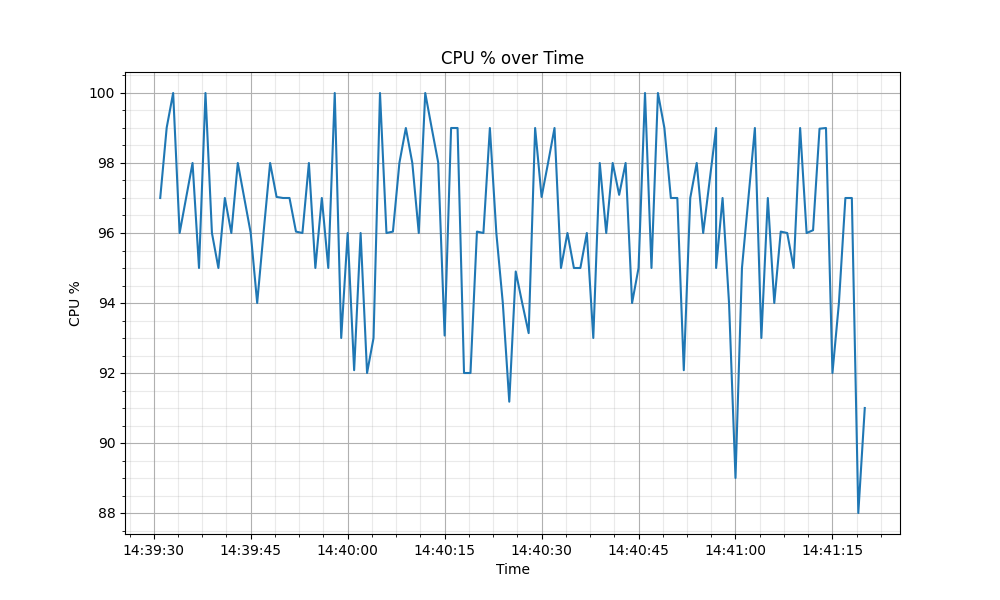
\includegraphics[width=\textwidth]{image/cpu_usage.png}
Применяем все настройки, как для \textit{fft}. Ставим приоритет 19, пробуем разные политики планирования (самой выгодной опять оказалась NORMAL), закреплем процессы за конкретными процессорами, отключаем графический интерфейс.\\
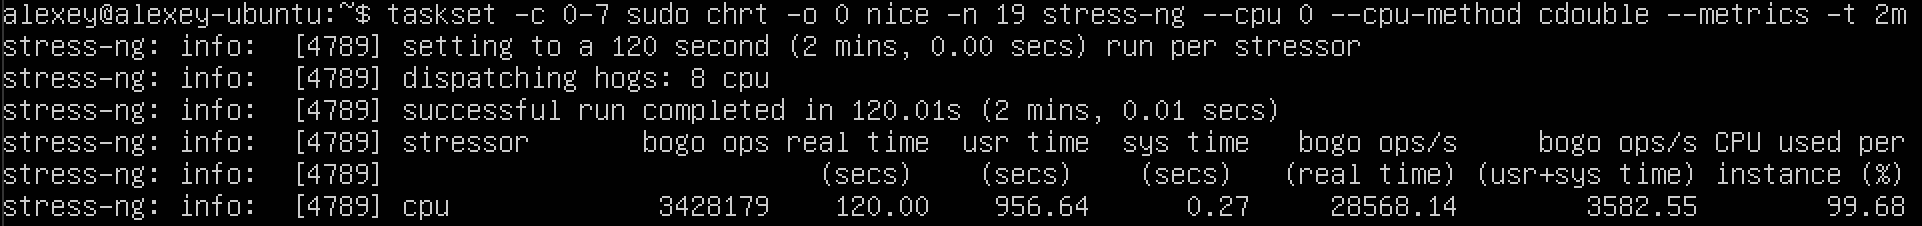
\includegraphics[width=\textwidth]{image/cpu-cdouble-max.png}
Итого с \textbf{1'844'831} bogo ops мы повысили производительность до \textbf{3'428'179} bogo ops.\\
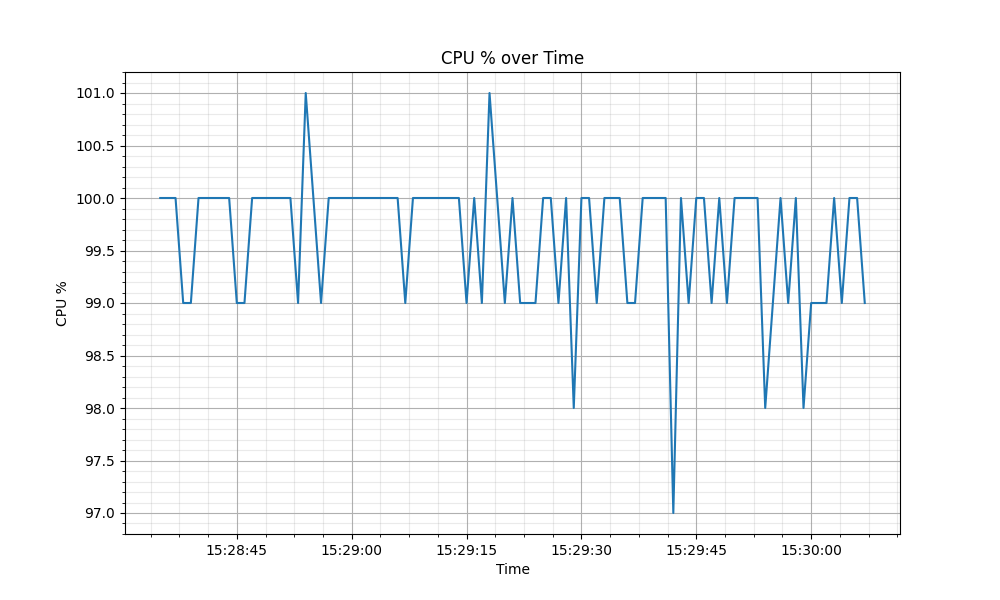
\includegraphics[width=\textwidth]{image/cpu_usage_max.png}

\subsection{Дополнительные команды для анализа, если интересно}
\subsubsection{turbostat}
\begin{verbatim}
alexey@alexey-ubuntu:~$ sudo turbostat
turbostat version 2022.10.04 - Len Brown <lenb@kernel.org>
Kernel command line: BOOT_IMAGE=/boot/vmlinuz-6.2.0-35-generic root=UUID=9331bdb4-8632-46ca-9360-21d342336892 ro quiet splash vt.handoff=7
CPUID(0): GenuineIntel 0x16 CPUID levels
CPUID(1): family:model:stepping 0x6:8e:a (6:142:10) microcode 0x0
CPUID(0x80000000): max_extended_levels: 0x80000008
CPUID(1): SSE3 - - - - TSC MSR - HT -
CPUID(6): No-APERF, No-TURBO, DTS, PTM, No-HWP, No-HWPnotify, No-HWPwindow, No-HWPepp, No-HWPpkg, No-EPB
cpu1: MSR_IA32_MISC_ENABLE: 0x00001810 (No-TCC No-EIST No-MWAIT PREFETCH TURBO)
CPUID(7): No-SGX No-Hybrid
CPUID(0x15): eax_crystal: 2 ebx_tsc: 192 ecx_crystal_hz: 0
TSC: 2304 MHz (24000000 Hz * 192 / 2 / 1000000)
CPUID(0x16): base_mhz: 2300 max_mhz: 3800 bus_mhz: 100
cpu1: MSR_MISC_PWR_MGMT: 0x00000000 (ENable-EIST_Coordination DISable-EPB DISable-OOB)
RAPL: inf sec. Joule Counter Range, at 0 Watts
cpu1: MSR_PLATFORM_INFO: 0x00001700
0 * 100.0 = 0.0 MHz max efficiency frequency
23 * 100.0 = 2300.0 MHz base frequency
cpu1: MSR_IA32_POWER_CTL: 0x00000000 (C1E auto-promotion: DISabled)
cpu1: MSR_PKG_CST_CONFIG_CONTROL: 0x00000000 (UNlocked, pkg-cstate-limit=0 (pc0))
/dev/cpu_dma_latency: 2000000000 usec (default)
current_driver: acpi_idle
current_governor: menu
current_governor_ro: menu
cpu1: POLL: CPUIDLE CORE POLL IDLE
cpu1: C1: ACPI HLT
NSFOD /sys/devices/system/cpu/cpu1/cpufreq/scaling_driver
cpu1: MSR_MISC_FEATURE_CONTROL: 0x00000000 (L2-Prefetch L2-Prefetch-pair L1-Prefetch L1-IP-Prefetch)
cpu0: MSR_RAPL_POWER_UNIT: 0x00000000 (1.000000 Watts, 1.000000 Joules, 0.000977 sec.)
cpu0: MSR_PKG_POWER_INFO: 0x00000000 (0 W TDP, RAPL 0 - 0 W, 0.000000 sec.)
cpu0: MSR_PKG_POWER_LIMIT: 0x00000000 (UNlocked)
cpu0: PKG Limit #1: DISabled (0.000 Watts, 0.000977 sec, clamp DISabled)
cpu0: PKG Limit #2: DISabled (0.000 Watts, 0.000977* sec, clamp DISabled)
cpu0: MSR_VR_CURRENT_CONFIG: 0x00000000
cpu0: PKG Limit #4: 0.000000 Watts (UNlocked)
cpu0: MSR_DRAM_POWER_LIMIT: 0x00000000 (UNlocked)
cpu0: DRAM Limit: DISabled (0.000 Watts, 0.000977 sec, clamp DISabled)
cpu0: MSR_PP0_POLICY: 0
cpu0: MSR_PP0_POWER_LIMIT: 0x00000000 (UNlocked)
cpu0: Cores Limit: DISabled (0.000 Watts, 0.000977 sec, clamp DISabled)
cpu0: MSR_PP1_POLICY: 0
cpu0: MSR_PP1_POWER_LIMIT: 0x00000000 (UNlocked)
cpu0: GFX Limit: DISabled (0.000 Watts, 0.000977 sec, clamp DISabled)
cpu0: MSR_IA32_TEMPERATURE_TARGET: 0x00c80000 (200 C)
cpu0: MSR_IA32_PACKAGE_THERM_STATUS: 0x00160000 (178 C)
cpu0: MSR_IA32_PACKAGE_THERM_INTERRUPT: 0x00000000 (200 C, 200 C)
cpu1: MSR_PKGC3_IRTL: 0x00000000 (NOTvalid, 0 ns)
cpu1: MSR_PKGC6_IRTL: 0x00000000 (NOTvalid, 0 ns)
cpu1: MSR_PKGC7_IRTL: 0x00000000 (NOTvalid, 0 ns)
cpu1: MSR_PKGC8_IRTL: 0x00000000 (NOTvalid, 0 ns)
cpu1: MSR_PKGC9_IRTL: 0x00000000 (NOTvalid, 0 ns)
cpu1: MSR_PKGC10_IRTL: 0x00000000 (NOTvalid, 0 ns)
turbostat: cpu1: perf instruction counter: No such file or directory
Can not set timer.
Core	CPU	TSC_MHz	IRQ	SMI	POLL	C1	POLL%	C1%	CPU%c1	CPU%c3	CPU%c6	CPU%c7	CoreTmp	PkgTmp	Totl%C0Any%C0	GFX%C0	CPUGFX%	PkgWatt	CorWatt	GFXWatt	RAMWatt	PKG_%	RAM_%
-	-	2303	9689	0	0	0	0.00	0.00	100.00	0.00	0.00	0.00	178	178	0.00	0.00	0.00	0.00	3675512670100409344.00	806784702202014720.00	749353303706249472.00	720671569983397120.00	74608482807378272.00	67477450522557608.00
0	0	2304	1194	0	0	0	0.00	0.00	100.00	0.00	0.00	0.00	178	178	0.00	0.00	0.00	0.00	3681394793109877248.00	808075843679804672.00	750552534590639488.00	721824899927965824.00	74727882823869232.00	67585438359891904.00
1	1	2304	1216	0	0	0	0.00	0.00	100.00	0.00	0.00	0.00	178
2	2	2304	1185	0	0	0	0.00	0.00	100.00	0.00	0.00	0.00	178
3	3	2304	1191	0	0	0	0.00	0.00	100.00	0.00	0.00	0.00	178
4	4	2304	1195	0	0	0	0.00	0.00	100.00	0.00	0.00	0.00	178
5	5	2304	1184	0	0	0	0.00	0.00	100.00	0.00	0.00	0.00	178
6	6	2304	1295	0	0	0	0.00	0.00	100.00	0.00	0.00	0.00	178
7	7	2304	1229	0	0	0	0.00	0.00	100.00	0.00	0.00	0.00	178
\end{verbatim}
\subsubsection{uptime}
\begin{verbatim}
alexey@alexey-ubuntu:~$ uptime
17:50:29 up  1:07,  1 user,  load average: 8,11, 4,01, 2,21
\end{verbatim}
\subsubsection{numastat}
\begin{verbatim}
alexey@alexey-ubuntu:~$ numastat -cm

Per-node system memory usage (in MBs):
Token SwapCached not in hash table.
Token SecPageTables not in hash table.
Token FileHugePages not in hash table.
Token FilePmdMapped not in hash table.
                 Node 0 Total
                 ------ -----
MemTotal           1952  1952
MemFree             196   196
MemUsed            1755  1755
Active              558   558
Inactive            719   719
Active(anon)        175   175
Inactive(anon)      436   436
Active(file)        383   383
Inactive(file)      283   283
Unevictable         133   133
Mlocked              20    20
Dirty                 0     0
Writeback             0     0
FilePages           819   819
Mapped              177   177
AnonPages           604   604
Shmem               129   129
KernelStack          10    10
PageTables           18    18
NFS_Unstable          0     0
Bounce                0     0
WritebackTmp          0     0
Slab                242   242
SReclaimable        130   130
SUnreclaim          112   112
AnonHugePages         0     0
ShmemHugePages        0     0
ShmemPmdMapped        0     0
HugePages_Total       0     0
HugePages_Free        0     0
HugePages_Surp        0     0
KReclaimable        130   130

\end{verbatim}